%%%%%%%%%%%%%%%%%%%%%%%%%%%%%%%%%%%%%%%%%%%%%%%%%%%%%%%%%%%%
% CHAPTER 3 – REQUIREMENT ANALYSIS
%%%%%%%%%%%%%%%%%%%%%%%%%%%%%%%%%%%%%%%%%%%%%%%%%%%%%%%%%%%%

\chapter{Requirement Analysis}

%===========================================================
\section{Introduction to Requirement Analysis}
%===========================================================

This chapter presents a structured and formal specification of system requirements for the Let's Go ride-sharing application. The purpose of this chapter is to clearly define what the system shall accomplish before proceeding to the system design phase. The requirements documented in this chapter serve as a contractual foundation for implementation, validation, and system testing.

The requirement analysis includes requirement elicitation techniques, identification of stakeholders, use case modeling, functional requirements, non-functional requirements, and external interface requirements. All requirements are written in measurable and testable format using standard requirement engineering principles.

%===========================================================
\section{Requirement Elicitation Techniques}
%===========================================================

This section describes the techniques used to gather and refine system requirements. Requirement elicitation ensures alignment between stakeholder expectations and system capabilities.

Requirements for the Let's Go project were identified using the following techniques:

\begin{itemize}
    \item \textbf{Stakeholder interviews} with potential drivers, passengers, and administrators to capture user expectations, pain points, and desired features.
    \item \textbf{Literature review} of existing ride-sharing platforms (BlaBlaCar, InDrive, Bykea) and academic research on carpooling systems.
    \item \textbf{Analysis of existing solutions} to identify functional gaps, such as lack of route-based matching and cultural preferences.
    \item \textbf{Dataset examination} for the machine learning module, studying travel patterns and user behavior to define recommendation features.
    \item \textbf{Observation of workflow processes} in current transportation services to understand manual verification, payment handling, and dispute resolution needs.
\end{itemize}

%===========================================================
\section{User Classes and Characteristics}
%===========================================================

This section identifies different user categories interacting with the Let's Go system. Each user class is defined along with their responsibilities, access privileges, and technical proficiency level. This classification supports role-based access control and requirement mapping.

\begin{table}[htbp]
\centering
\caption{User Classes and Characteristics}
\begin{tabularx}{\textwidth}{|p{3cm}|X|p{3cm}|}
\hline
\rowcolor{lightgray!30}
\textbf{User Class} & \textbf{Description} & \textbf{Technical Level} \\
\hline
Administrator & Manages user verification, dispute resolution, financial analytics, and system configuration via a web-based admin panel. & Advanced \\
\hline
Driver & Creates rides, manages vehicles, accepts bookings, coordinates with passengers, and completes trips. Must undergo document verification. & Intermediate \\
\hline
Passenger & Searches and books rides, communicates with drivers, makes payments, and provides ratings. & Basic \\
\hline
External System & Third-party services such as Maps API, Notification Service (FCM, SMS, email), and LLM API for chatbot integration. & Technical \\
\hline
\end{tabularx}
\end{table}

%===========================================================
\section{System Overview}
%===========================================================

The proposed Let's Go system operates within a structured architectural environment designed to support modular interaction between user interfaces, processing logic, and data storage. The system supports role-based interactions and ensures secure communication between internal modules and external services.

The overall architecture follows a \textbf{three-tier client-server model}:
\begin{itemize}
    \item \textbf{Presentation Tier:} Cross-platform Flutter mobile applications for passengers and drivers, and a web-based admin console (HTML/CSS/JavaScript).
    \item \textbf{Application Tier:} Django backend with REST-style JSON APIs for core features (auth, rides, bookings, chat, live tracking, safety, Admin, and ML recommendations). Mobile clients implement real-time behavior using periodic HTTP updates.
    \item \textbf{Data Tier:} PostgreSQL (Supabase) for transactional data and object storage for documents.
\end{itemize}

The system boundary includes all internal modules, user interfaces, data processing components, and integrated third-party services (Maps, Notifications, LLM). External entities interact with the system via well-defined APIs.

%===========================================================
\section{Use Case Model}
%===========================================================

The use case model represents high-level system interactions between actors and system functionalities. It defines system boundaries and captures functional behavior from a user perspective.

%-----------------------------------------------------------------
\subsection{Use Case Diagram}
%-----------------------------------------------------------------

The Let's Go system encompasses 25 use cases covering registration, vehicle management, ride creation, booking, ride execution, safety, disputes, ML recommendations, chatbot support, and manual payment. The following diagrams illustrate the overall system and thematic groupings.

\begin{figure}[htbp]
    \centering
    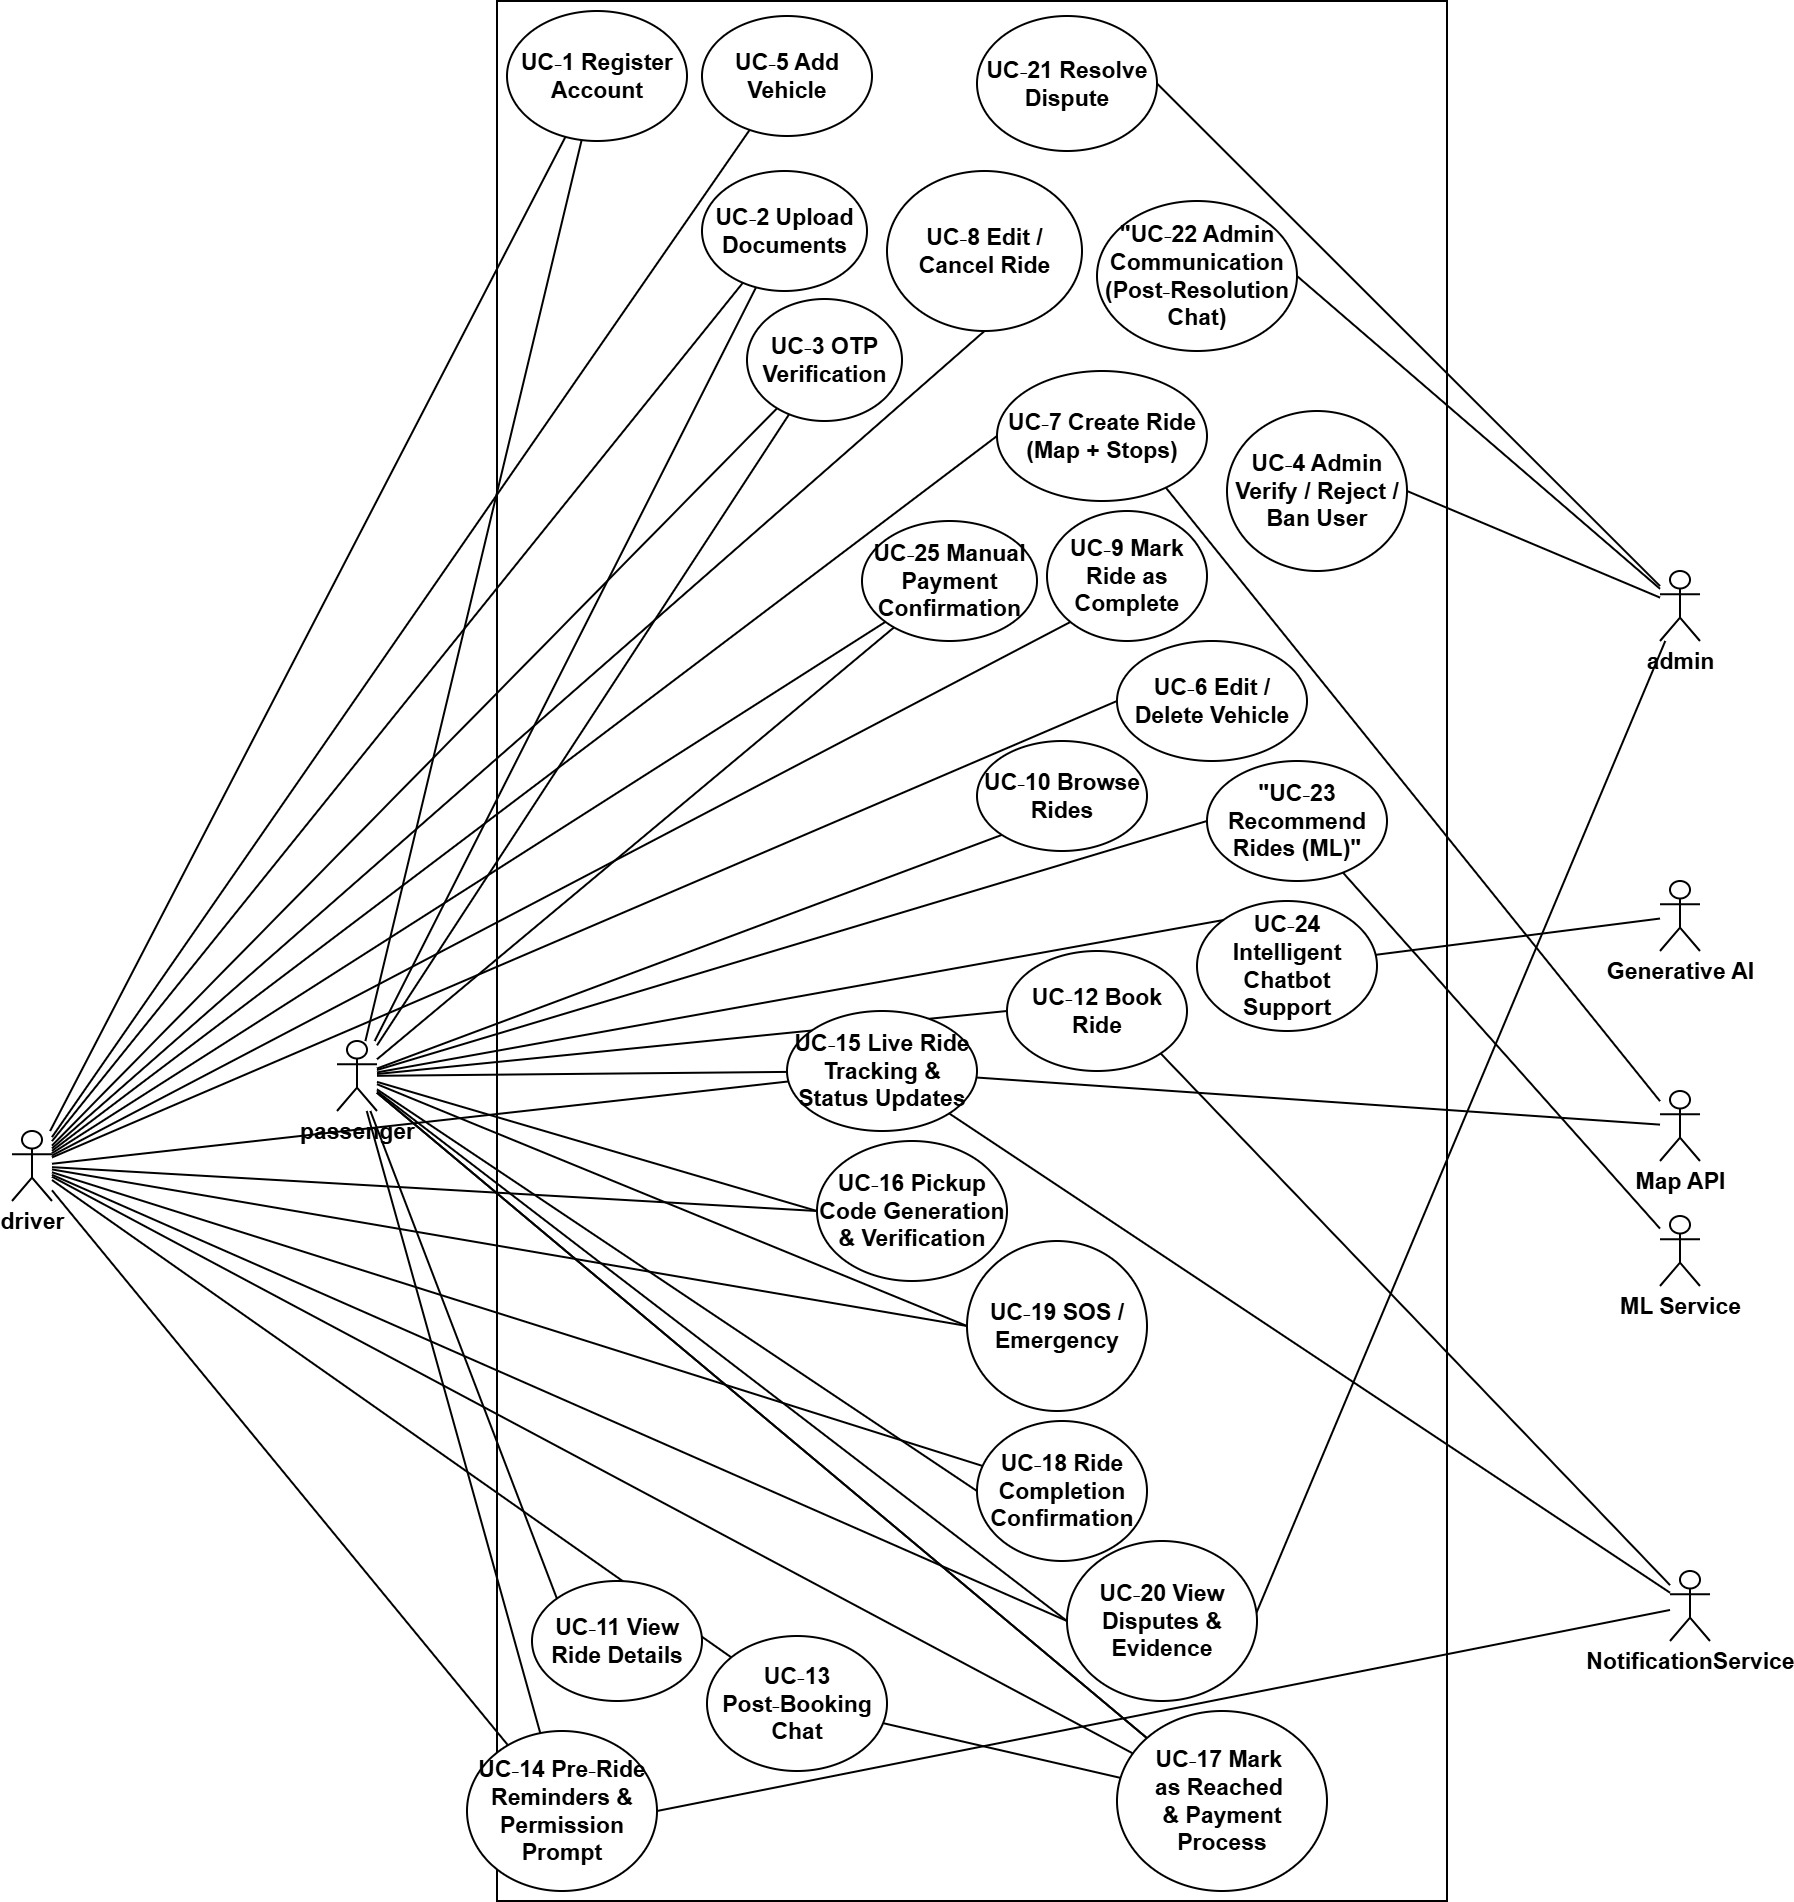
\includegraphics[width=\textwidth,keepaspectratio]{assets/master_uc.jpg}
    \caption{Master Use Case Diagram for the Let's Go system, covering all 25 use cases and the interactions between Driver, Passenger, Admin, and secondary Service APIs.}
    \label{fig:master_uc}
\end{figure}

\begin{figure}[htbp]
    \centering
    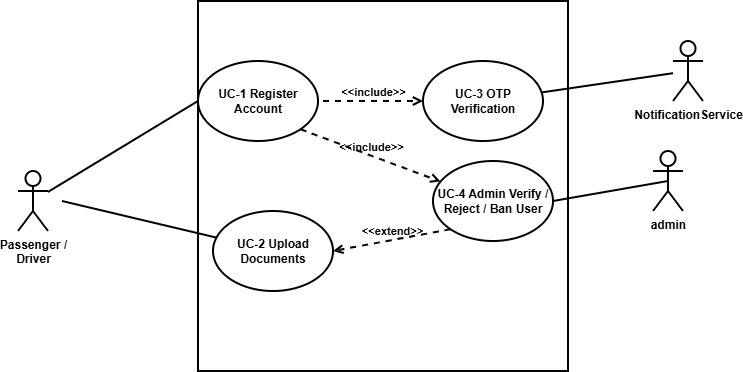
\includegraphics[width=0.8\textwidth,keepaspectratio,height=0.8\textheight]{assets/reg_verification_uc.jpg}
    \caption{Registration and Verification Theme: Illustrates the flow from account creation and multi-channel OTP verification to manual Admin identity approval.}
    \label{fig:registration_uc}
\end{figure}

\begin{figure}[htbp]
    \centering
    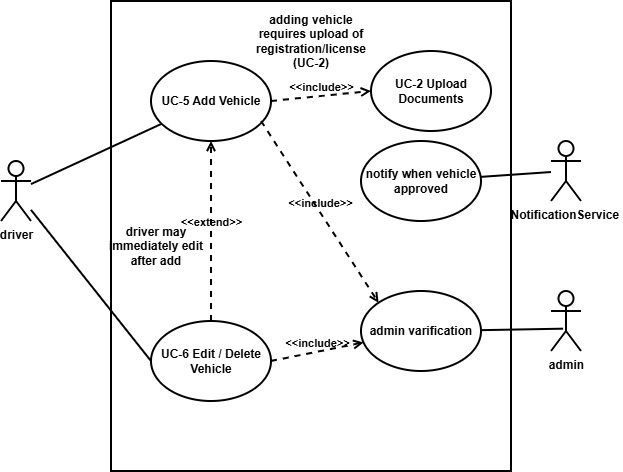
\includegraphics[width=0.8\textwidth,keepaspectratio,height=0.8\textheight]{assets/vehicle_management_uc.jpg}
    \caption{Vehicle Management: Covers the lifecycle of driver vehicle registration, including 2-wheel/4-wheel constraints and maintenance.}
    \label{fig:vehicle_uc}
\end{figure}

\begin{figure}[htbp]
    \centering
    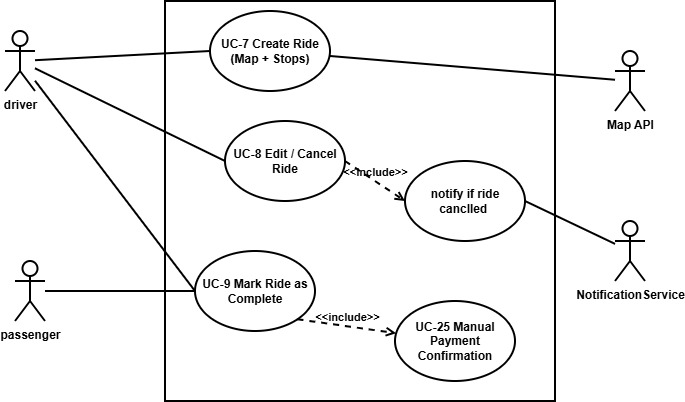
\includegraphics[width=0.8\textwidth,keepaspectratio,height=0.8\textheight]{assets/ride_management_uc.jpg}
    \caption{Ride Management: Detailed driver-side ride lifecycle from route-based creation to manual completion marking.}
    \label{fig:ride_mgmt_uc}
\end{figure}

\begin{figure}[htbp]
    \centering
    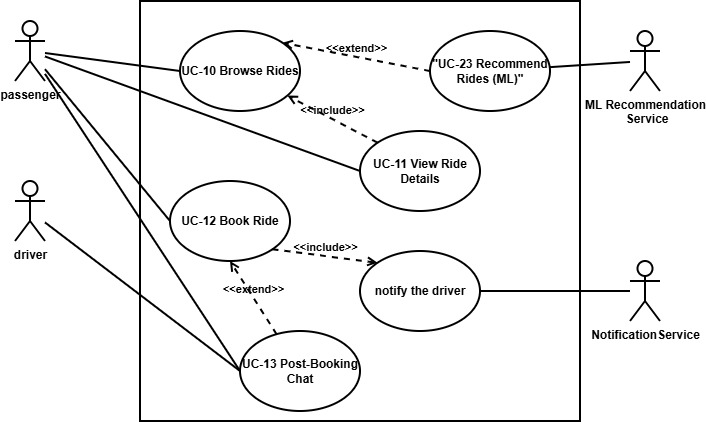
\includegraphics[width=0.8\textwidth,keepaspectratio,height=0.8\textheight]{assets/discovery_booking_uc.jpg}
    \caption{Discovery and Booking: The passenger search process, seat-locking mechanism, and post-booking coordination channels.}
    \label{fig:booking_uc}
\end{figure}

\begin{figure}[htbp]
    \centering
    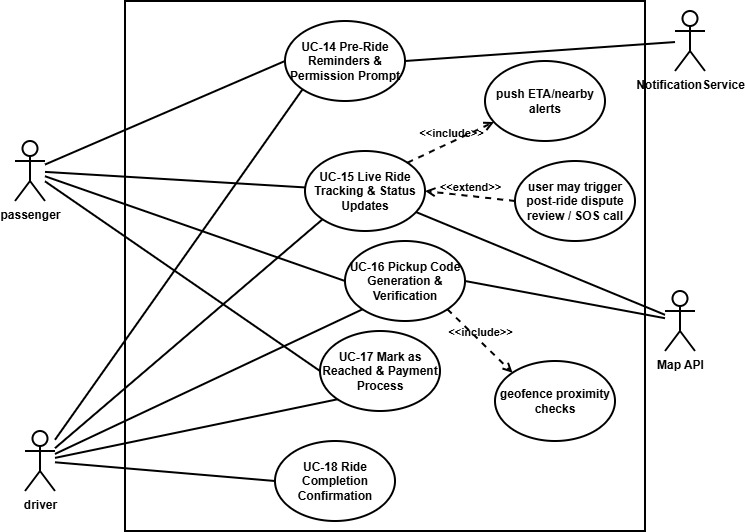
\includegraphics[width=0.8\textwidth,keepaspectratio,height=0.8\textheight]{assets/ride_execution_uc.jpg}
    \caption{Ride Execution Phase: Focuses on live GPS tracking, geofenced pickup code (OTP) verification, and arrival confirmations.}
    \label{fig:execution_uc}
\end{figure}

\begin{figure}[htbp]
    \centering
    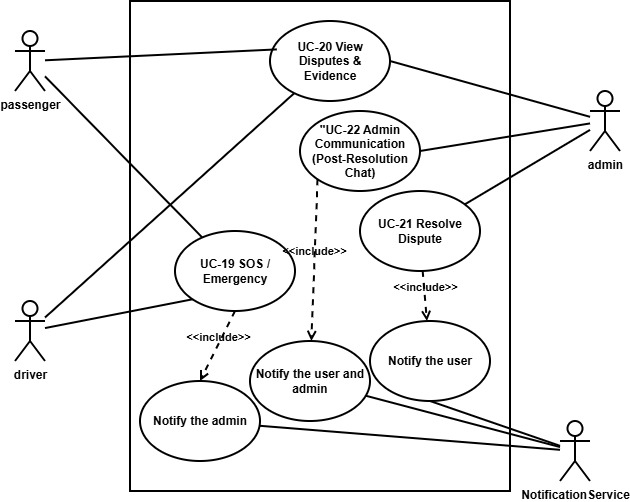
\includegraphics[width=0.8\textwidth,keepaspectratio,height=0.8\textheight]{assets/safety_disputes_uc.jpg}
    \caption{Safety and Disputes: Workflow for SOS alerts, emergency contact escalation, and admin audit of immutable evidence.}
    \label{fig:safety_uc}
\end{figure}

\begin{figure}[htbp]
    \centering
    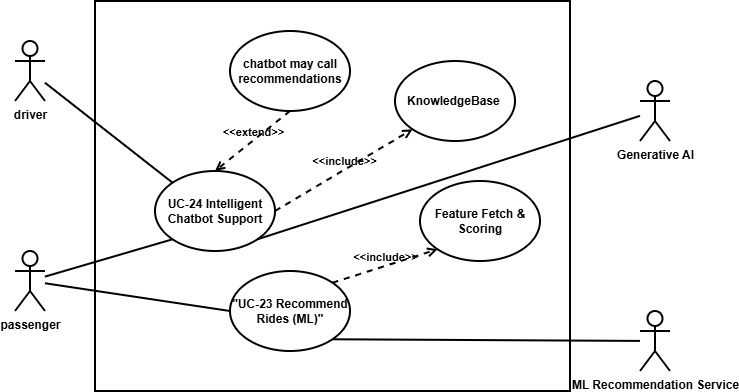
\includegraphics[width=0.8\textwidth,keepaspectratio,height=0.8\textheight]{assets/ml_chatbot_uc.jpg}
    \caption{AI/ML Features: Automated content-based ride recommendations and intelligent support via the Generative AI knowledge base.}
    \label{fig:ai_uc}
\end{figure}

\begin{figure}[htbp]
    \centering
    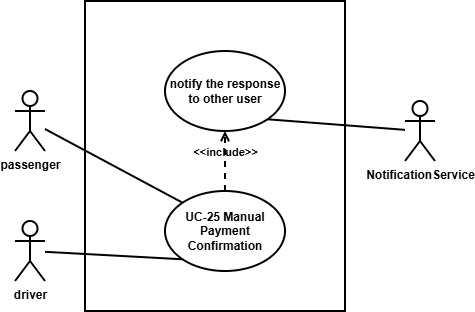
\includegraphics[width=0.8\textwidth,keepaspectratio,height=0.8\textheight]{assets/payment_uc.jpg}
    \caption{Manual Payment Flow: Two-step manual verification process for external fund transfers (Cash/Bank/QR).}
    \label{fig:payment_uc}
\end{figure}

\clearpage

%-----------------------------------------------------------------
\subsection{Use Case Descriptions}
%-----------------------------------------------------------------

This section provides detailed tabular specifications of all major use cases. These use cases form the basis for deriving functional requirements. They are organized by thematic modules.

%============================================================================
\subsubsection{Registration \& Verification (UC-1 to UC-4)}
%============================================================================

% ============================================================================
% Use Case UC-1: Register Account
% ============================================================================

\begin{longtable}{|p{3.5cm}|p{12cm}|}
\hline
\rowcolor{lightgray!30}
\textbf{Field} & \textbf{Value} \\
\hline
\endfirsthead
\hline
\rowcolor{lightgray!30}
\textbf{Field} & \textbf{Value} \\
\hline
\endhead
\hline
\endfoot
Use Case ID & UC-1 \\
\hline
Use Case Name & Register Account \\
\hline
Actors & 
\textbf{Primary Actor:} Unverified User

\textbf{Secondary Actors:} Notification Service (email/SMS), Admin (implicit actor for later verification), Chatbot (optional help) \\
\hline
Description & 
An Unverified User registers a new account by providing personal details and optional driver/bank data, uploads required documents/images, receives OTPs via email and SMS, and completes OTP verification. After successful OTP verification the account state is set to \textit{Pending Admin Verification}. The use case ensures that the system collects all data needed for identity checks and onboarding. \\
\hline
Trigger & 
User opens the app or web signup page and chooses \textit{Create Account / Sign Up}. \\
\hline
Normal (Basic) Flow (Main Success Scenario) &
Unverified User opens the Registration screen and fills in the registration form with required fields (name, username, email, password + confirm password, address, phone number, CNIC, gender).

User may optionally enter bank account number and bank name (both required if one is supplied) and/or driving license number.

User uploads the required images (profile photo, live photo, CNIC front/back). If driving license number was entered, license front/back images were uploaded. If bank transfer/QR will be used, account QR is uploaded. The UI validates image formats and sizes before uploading.

User submits the registration form. Client performs basic validation (required fields, password strength, unique username/email check via quick server call).

Server validates the submission, creates a provisional user record with status OTP\_VERIFICATION\_PENDING, and stores the uploaded files securely.

System generates two OTPs (one for email, one for phone) and sends them through Notification Service (email + SMS). Each OTP has a 5-minute expiry.

System shows OTP entry screen to user. Users enter both OTPs.

Server verifies OTPs; if both are valid and not expired, server sets user state to PENDING\_ADMIN\_VERIFICATION and returns success.

System displays a confirmation page: ``OTP verified --- your account is pending admin verification. You will be notified when verification completes.''

User is redirected to login screen (or offered to log in after admin verifies). \\
\hline
Preconditions & 
User has a device with an active internet connection.

Users have a valid email address and phone number to receive OTPs. \\
\hline
Postconditions & 
On success: user account created with PENDING\_ADMIN\_VERIFICATION status and audit logs recorded.

On failure: user remains unverified; errors reported to user; partial data retained per retention policy. \\
\hline
Alternate Flows \& Exceptions & 
\textbf{A1 --- Missing Required Field / Client-side validation fails}

If the user omits required fields or client-side validation fails, display inline errors and block submission until corrected. Return to step 1.

\textbf{A2 --- Server-side validation failure (e.g., duplicate email/username)}

If server detects duplicate username/email or invalid CNIC format, return error to user with specific message. User corrects input and resubmits.

\textbf{A3 --- Image upload fails (format/size or network error)}

Inform user which image failed and why (wrong format, too large). Allow reattempt. If network error occurs, allow resume/retry.

\textbf{A4 --- OTP expired / wrong OTP}

If an OTP is expired or incorrect, it shows specific error. Allow users to request resend. Return to OTP entry step.

\textbf{A5 --- OTP delivery failure (SMS/email gateway problem)}

If Notification Service reports failure, show a message suggesting retrying and optionally use alternate channel (send email if SMS failed). Log the failure and increment a metric for admin review.

\textbf{A6 --- User abandons signup.}

If user closes app or times out, provisional data is retained per retention policy. \\
\hline
Business Rules (BR) & 
\textbf{BR-1:} OTP expiration = 5 minutes.

\textbf{BR-2:} If bank account number is provided, bank name is mandatory and vice versa.

\textbf{BR-3:} Username and email must be unique.

\textbf{BR-4:} Driving license images are required only if driving license number field is provided.

\textbf{BR-5:} Uploaded images must meet size and format constraints (configurable); reject otherwise. \\
\hline
Assumptions & 
Notification Service (email/SMS) is available and operational.

Users will have access to the email and phone provided for OTP reception.

CNIC format rules and validation logic are defined elsewhere and available to the system. \\
\hline
\caption{UC-1: Register Account}
\end{longtable}

% ============================================================================
% Use Case UC-2: Upload Documents
% ============================================================================

\begin{longtable}{|p{3.5cm}|p{12cm}|}
\hline
\rowcolor{lightgray!30}
\textbf{Field} & \textbf{Value} \\
\hline
\endfirsthead
\hline
\rowcolor{lightgray!30}
\textbf{Field} & \textbf{Value} \\
\hline
\endhead
\hline
\endfoot
Use Case ID & UC-2 \\
\hline
Use Case Name & Upload Documents \\
\hline
Actors & 
\textbf{Primary Actor:} Unverified User / User (during profile completion or driver onboarding)

\textbf{Secondary Actors:} Notification Service (for confirmations), Admin (viewer during verification), Chatbot (optional help) \\
\hline
Description & 
A user uploads required identity and vehicle documents (profile photo, live photo, CNIC front/back, account QR, driving license front/back if applicable, and vehicle images when adding a vehicle). The system validates file formats and sizes, stores files securely, and links them to the user or vehicle records. Admins later review these documents as part of verification. \\
\hline
Trigger & 
User navigates to the document-upload screen during registration, profile editing, or while adding a vehicle and initiates the upload action. \\
\hline
Normal (Basic) Flow (Main Success Scenario) &
User navigates to the Upload Documents section (either during registration flow or later via profile → documents).

UI displays required and optional document slots with accepted formats and size limits (e.g., JPG/PNG, max dimensions/MB).

User selects a document slot (e.g., CNIC front) and chooses/upload an image from device or camera.

Client performs lightweight checks (file type, file size) and displays immediate validation errors if invalid.

Client uploads files to server (multipart/form-data) with metadata: user\_id, document\_type, timestamp, optional vehicle\_id.

Server validates the payload (file type, file signature where possible, size, image dimensions) and stores the file.

Server creates a document record linking file location, document type, user\_id (or vehicle\_id), upload timestamp and status PENDING\_REVIEW.

Server returns success; UI shows uploaded thumbnail and status Uploaded - pending admin review (if applicable). Notification Service optionally sends confirmation (email/in-app).

Admin can later view these uploaded documents in Admin portal as part of FR-2 verification flows. \\
\hline
Preconditions & 
User is authenticated (in profile flow) or in registration flow with session state.

The client device has camera or file access and internet connectivity. \\
\hline
Postconditions & 
Document saved and linked to user/vehicle record.

Document status recorded (PENDING\_REVIEW / APPROVED / REJECTED).

Notification (optional) sent to user confirming upload. \\
\hline
Alternate Flows \& Exceptions & 
\textbf{A1 --- Client-side Validation Failure (wrong format / too large)}

If client-side validation fails, show clear error and prevent upload. Provide guidance on acceptable format/size. Return to step 3.

\textbf{A2 --- Upload Interruption / Network Failure}

If upload fails mid-transfer, allow retry and resume where possible. Keep a temporary client-side copy until successful. Log transfer failures.

\textbf{A3 --- Server-side Validation Failure (malformed file/signature mismatch)}

Server rejects file, returns an error with reason (e.g., ``file appears corrupted''), and notifies user to re-upload.

\textbf{A4 --- Duplicate or Previously Uploaded Document}

If user uploads a document of the same type and the previous one exists, UI shows both with timestamps and marks the latest as current or allows user to replace. Business rule governs replacement (e.g., replacing CNIC requires admin re-verification).

\textbf{A5 --- Unauthorized Upload Attempt}

If an unauthenticated or unauthorized client attempts upload, server rejects with 401/403. \\
\hline
Business Rules (BR) & 
\textbf{BR-1:} Accepted file formats: JPG, PNG (configurable).

\textbf{BR-2:} Max file size: 5 MB (configurable) reject larger files.

\textbf{BR-3:} Driving license images required if license number is provided.

\textbf{BR-4:} Account QR required if the user opts for bank transfer payouts.

\textbf{BR-5:} Replace/overwrite policy: uploading a new CNIC or license image sets the document status to PENDING\_REVIEW and triggers re-verification by Admin. \\
\hline
Assumptions & 
Storage service is available.

Admins have a secure admin portal to view/review documents. \\
\hline
\caption{UC-2: Upload Documents}
\end{longtable}

\begin{longtable}{|p{3.5cm}|p{12cm}|}
\hline
\rowcolor{lightgray!30}
\textbf{Field} & \textbf{Value} \\
\hline
\endfirsthead
\hline
\rowcolor{lightgray!30}
\textbf{Field} & \textbf{Value} \\
\hline
\endhead
\hline
\endfoot
Use Case ID & UC-3 \\
\hline
Use Case Name & OTP Verification \\
\hline
Actors &
\textbf{Primary Actor:} Unverified User (or User performing email/phone change)

\textbf{Secondary Actors:} Notification Service (email/SMS), Admin (for logging/alerts), Chatbot (optional help) \\
\hline
Description &
The system validates one-time passwords (OTPs) sent to a user's email and phone to confirm ownership of contact channels. Successful OTP verification transitions the account to PENDING\_ADMIN\_VERIFICATION. OTPs are short-lived and subject to resend/attempt limits to prevent abuse. \\
\hline
Trigger &
System sends OTPs after registration submission or when a user requests an email/phone change that requires re-verification; user navigates to OTP entry screen. \\
\hline
Normal (Basic) Flow (Main Success Scenario) &
After registration (UC-1) or contact-change request, system generates an email OTP and a phone (SMS) OTP and sends them via Notification Service.

System records OTPs in secure store with timestamps, expiry (5 minutes default), and attempt counters.

User receives OTPs and navigates to the OTP entry screen.

User enters both OTP codes and submits them.

Server verifies OTPs; if both are valid and not expired, server sets user state to PENDING\_ADMIN\_VERIFICATION and returns success.

System displays success message and redirects user to next appropriate screen (login or profile). \\
\hline
Preconditions &
User has completed registration form or requested contact information change.

User has access to the provided email and phone for OTP reception.

Notification Service is operational. \\
\hline
Postconditions &
\textbf{On success:} User account state transitions to PENDING\_ADMIN\_VERIFICATION.

\textbf{On failure:} User remains in current state; OTP attempts logged.

OTP verification event recorded in audit logs. \\
\hline
Alternate Flows \& Exceptions &
\textbf{A1 --- Wrong OTP Entered}

If user enters incorrect OTP, system displays error message showing remaining attempts. User can retry within attempt limits.

\textbf{A2 --- OTP Expired}

If OTP has expired (5 minutes), system informs user and offers option to resend new OTPs.

\textbf{A3 --- Exceeded Attempt Limit}

If user exceeds maximum allowed OTP attempts (default 5), system locks OTP verification for cooldown period (default 15 minutes) and requires support contact.

\textbf{A4 --- OTP Delivery Failure}

If Notification Service fails to deliver OTP via email or SMS, system logs failure, alerts admin, and offers alternative delivery method.

\textbf{A5 --- Resend OTP Requested}

User requests OTP resend; system generates new OTPs (invalidating previous ones) and sends via Notification Service, subject to resend limits.

\textbf{A6 --- User Cancels/Abandons}

If users leave OTP screen without completing, OTPs remain valid until expiry; server may garbage-collect unused OTPs per retention policy. \\
\hline
Business Rules (BR) &
OTP expiry default = 5 minutes (admin-configurable).

Max OTP verification attempts per OTP code = 5 (admin-configurable). On exceed, impose cooldown (e.g., 15 minutes) or require support.

Max OTP resend per time window (e.g., 3 per hour) to avoid abuse.

OTPs are single-use; resending invalidates prior OTPs.

Do not disclose which OTP (email or SMS) failed in error messages to avoid user enumeration; show generic "OTP invalid" with remaining attempts.

Record OTP generation and verification attempts for audit and fraud detection.

For contact-change workflows, require re-verification of the changed contact before applying the change. \\
\hline
Assumptions &
Users can access the email and phone they provide.

Time drift between server and client is negligible for 5-minute expiry; server time is authoritative.

Notification Service has reliable delivery mechanisms for email and SMS. \\
\hline
\caption{UC-3: OTP Verification}
\end{longtable}

\begin{longtable}{|p{3.5cm}|p{12cm}|}
\hline
\rowcolor{lightgray!30}
\textbf{Field} & \textbf{Value} \\
\hline
\endfirsthead
\hline
\rowcolor{lightgray!30}
\textbf{Field} & \textbf{Value} \\
\hline
\endhead
\hline
\endfoot
Use Case ID & UC-4 \\
\hline
Use Case Name & Admin Verify / Reject / Ban User \\
\hline
Actors &
\textbf{Primary Actor:} Admin

\textbf{Secondary Actors:}

User (awaiting verification)

Notification Service (for sending approval/rejection messages) \\
\hline
Description &
This case defines how the admin reviews newly registered users and their submitted documents, then decides to verify, reject, or ban them. Verification grants the user full access; rejection denies access with feedback; banning permanently prevents future re-registration using the same CNIC. The admin also handles user disputes and can create new accounts upon special requests. \\
\hline
Trigger &
Admin logs into the admin panel and navigates to the User Verification section or receives an automated alert indicating new pending verifications. \\
\hline
Normal (Basic) Flow (Main Success Scenario) &
Admin opens the Admin Portal dashboard.

The system displays all registered users with status "Pending Admin Verification."

Admin selects a user to view details.

The system displays user information, including:

Name, Username, Email, Phone, CNIC, Gender, and Address

Uploaded documents: profile photo, CNIC front/back, live photo, and license (if any).

Admin reviews all details and ensures document authenticity.

Admin chooses Verify User and clicks confirm.

The system updates user status from Pending → Verified.

Notification Service sends approval notification via email/SMS.

The user gains full system access (login → dashboard). \\
\hline
Preconditions &
User has completed registration and OTP verification (UC-1, UC-3).

Admin is logged in.

System database and document storage are accessible. \\
\hline
Postconditions &
\textbf{On success:} User becomes active (verified) and can log in normally.

\textbf{On rejection:} User cannot log in until re-registration.

\textbf{On ban:} CNIC permanently blacklisted; login and registration disabled. \\
\hline
Alternate Flows \& Exceptions &
\textbf{A1 --- Rejection}

If admin finds incomplete or mismatched documents, they click Reject User. System prompts for a rejection reason. Admin enters a reason (e.g., "Invalid CNIC" or "Unreadable photo"). System sets user status to REJECTED. Notification Service sends rejection messages with reason. Users must re-register with corrected details (if allowed).

\textbf{A2 --- Ban (Permanent Block)}

If unethical behavior, fraud, or complaint is confirmed, admin selects Ban User. System prompts confirmation to permanently ban CNIC. Once confirmed, system adds CNIC to Banned List (blacklist), sets account status to BANNED, and restricts login and new registrations using the same CNIC. Notification Service informs the user of permanent ban and reason.

\textbf{A3 --- Dispute Resolution (Related Function)}

Admin navigates to Dispute Center to review any user complaints. Admin communicates with involved users and marks the dispute Resolved or to be resolved. The system updates dispute records accordingly.

\textbf{A4 --- Create Account (By Admin)}

Admin selects "Create User Account" manually (e.g., for support or test cases). Admin enters user details and uploads necessary documents. System creates verified accounts directly (bypassing OTP).

\textbf{A5 --- Verification Delay / Timeout}

If there is no verification action within 24 hours, system highlights delayed accounts in dashboard reminders or sends admin alerts. Admin proceeds to verify/reject after review. \\
\hline
Business Rules (BR) &
Verification must occur within 24 hours of registration submission.

Only Admins with Verification Privilege can approve or reject users.

Banned CNICs cannot be re-registered.

All verification/rejection/ban actions must log Admin ID, timestamp, and reason.

Notification Service must send messages within 2 minutes of decision.

Admin cannot verify users with missing mandatory documents.

Rejection does not delete the user record — keeps it for audit and future reapplication.

Verification changes are irreversible except by Super Admin override. \\
\hline
Assumptions &
Admins are trustworthy and trained to recognize fake or edited documents.

Network and storage systems are stable (document previews load correctly).

Notification Service can reach users reliably (email/SMS).

%============================================================================
\subsubsection{Vehicle Management (UC-5 to UC-6)}
%============================================================================ \\
\hline
\caption{UC-4: Admin Verify / Reject / Ban User}
\end{longtable}

\begin{longtable}{|p{3.5cm}|p{12cm}|}
\hline
\rowcolor{lightgray!30}
\textbf{Field} & \textbf{Value} \\
\hline
\endfirsthead
\hline
\rowcolor{lightgray!30}
\textbf{Field} & \textbf{Value} \\
\hline
\endhead
\hline
\endfoot
Use Case ID & UC-5 \\
\hline
Use Case Name & Add Vehicle \\
\hline
Actors &
\textbf{Primary Actor:} Driver (User role with verified license)

\textbf{Secondary Actors:}

Admin (may view vehicle during verification)

Notification Service (in-app/email confirmations) \\
\hline
Description &
A verified Driver who has provided a driving license shall be able to register one or more vehicles in their profile by entering vehicle metadata (model, variant, company, plate number, vehicle type, color, number of seats, engine/chassis numbers, fuel type, registration date, insurance expiry) and uploading required images (vehicle front, vehicle back, document/card). The system validates entries, enforces business rules (e.g., 2-wheeler seats fixed at 2), stores images securely, and links vehicles to the driver account. Optionally, vehicle uploads may trigger admin review depending on policy. \\
\hline
Trigger &
Driver navigates to Profile → Vehicle Management → Add Vehicle or is prompted to add a vehicle after entering a driving license number during registration/profile update. \\
\hline
Normal (Basic) Flow (Main Success Scenario) &
Driver navigates to "Add Vehicle" screen and clicks Add Vehicle.

UI displays the required form fields and accepts image slots with hints (image sizes/formats).

Driver fills in the form with:

Model Number (text)

Variant (optional)

Company Name (text)

Plate Number (text)

Vehicle Type (select: 2-wheeler / 4-wheeler)

Color (text/picker)

No. of Seats (if 4W; if 2W it is auto set to 2)

Engine Number (optional)

Chassis Number (optional)

Fuel Type (select petrol / diesel / CNG / electric / hybrid)

Registration Date (optional)

Insurance Expiry Date (optional)

Driver uploads required images: vehicle front, vehicle back, and registration/document card. Client validates formats and sizes.

Client submits the form. Client performs quick validation (required fields, plate format, seat rule for 2W).

Server validates input (plate uniqueness, enums, dates), stores vehicle record with status ACTIVE (or PENDING\_REVIEW if admin review policy enabled), and saves images to secure storage.

System links the vehicle entry to driver's user record.

System returns success and displays the new vehicle in the driver's profile listing. Optionally, Notification Service sends confirmation to driver (in-app/email).

If policy requires admin approval for vehicles, system sets PENDING\_REVIEW and notifies admin; once admin approves vehicle status changes to ACTIVE. \\
\hline
Preconditions &
Driver is authenticated and verified (license present) or has provided license number and completed OTPs (policy-dependent).

Storage and image processing services available. \\
\hline
Postconditions &
\textbf{On success:} vehicle record created and available for ride creation (unless awaiting admin approval).

\textbf{On failure:} no vehicle record created; error returned to driver. \\
\hline
Alternate Flows \& Exceptions &
\textbf{A1 --- Missing Required Field / Client Validation Fail}

If required fields missing or client-side validation fails (e.g., seat count omitted for 4W), show inline error and block submission.

\textbf{A2 --- Image Upload Failure / Format Error}

If image upload fails or format invalid, show error and allow retry. If server rejects due to malware or corruption, return explicit message.

\textbf{A3 --- Duplicate Plate / Uniqueness Conflict}

If plate number already exists in system and is associated with a different driver (possible theft/fraud), reject creation and notify admin automatically for manual review. If duplicate with same driver (re-adding), allow update or show existing record.

\textbf{A4 --- Business Rule Violation (2W seats not 2)}

If driver selects 2W and attempts to set seats other than 2, client must enforce seat=2 and block custom input; server rejects conflicting requests.

\textbf{A5 --- Driver lacks validated license.}

If the driver attempts to add a vehicle but does not have a license number on file or is not verified for driving, block the action and prompt them to add license info and wait for admin verification.

\textbf{A6 --- Admin Review Required}

If vehicle creation policy requires admin review (optional), set vehicle to PENDING\_REVIEW and notify admin. Driver cannot use vehicle for ride creation until approved (configurable). \\
\hline
Business Rules (BR) &
Only users with a driving license number on their profile can add vehicles.

2-wheeler (2W) must have No. of Seats = 2 (enforced).

Plate numbers must be unique across system; collisions trigger manual review.

Vehicle images must meet format (JPG/PNG) and size constraints; reject otherwise.

Deleting a vehicle that is associated with an active or past ride requires admin approval or is blocked (soft-delete recommended).

Any change to critical vehicle fields (plate number, registration expiry) must set vehicle status to PENDING\_REVIEW (configurable). \\
\hline
Assumptions &
Plate number validation rules (format per country) are defined and available.

Admin may optionally require manual review for vehicle documents depending on risk policy.

System keeps a vehicle change history for audits and disputes. \\
\hline
\caption{UC-5: Add Vehicle}
\end{longtable}

\begin{longtable}{|p{3.5cm}|p{12cm}|}
\hline
\rowcolor{lightgray!30}
\textbf{Field} & \textbf{Value} \\
\hline
\endfirsthead
\hline
\rowcolor{lightgray!30}
\textbf{Field} & \textbf{Value} \\
\hline
\endhead
\hline
\endfoot
Use Case ID & UC-6 \\
\hline
Use Case Name & Edit / Delete Vehicle \\
\hline
Actors &
\textbf{Primary Actor:} Driver (verified, with vehicle(s) registered)

\textbf{Secondary Actors:}

Admin (may be required for approvals when critical fields change)

Notification Service (in-app/email confirmations) \\
\hline
Description &
A verified Driver edits details of an existing vehicle (e.g., color, number of seats for 4W, insurance expiry) or requests deletion of a vehicle. The system validates edits, enforces business rules (e.g., 2W seats fixed = 2), may mark a vehicle as PENDING\_REVIEW for admin approval in certain cases, and prevents deletion of vehicles tied to active rides without admin intervention. \\
\hline
Trigger &
Driver selects a vehicle from their profile listing and chooses Edit or Delete. \\
\hline
Normal (Basic) Flow — Edit Vehicle &
Driver opens Profile → Vehicles and selects an existing vehicle.

Driver clicks Edit and the system presents the current vehicle details in an editable form.

Driver modifies allowed fields (e.g., color, insurance expiry, engine/chassis, number of seats for 4W).

Client validates basic constraints (required fields, date formats).

Driver submits changes.

Server validates business rules (e.g., if vehicle type is 2W, seats must be 2; plate uniqueness).

If edits are non-critical (e.g., color), server updates vehicle records, logs change (who/when) and returns success. Notification Service optionally notifies driver of successful update.

If edits are critical (plate number, registration info) or policy requires, server sets vehicle status to PENDING\_REVIEW and notifies admin to review. Driver is informed that vehicle is pending approval and may or may not be usable for new rides until approved. \\
\hline
Normal (Basic) Flow — Delete Vehicle &
Driver selects vehicle and clicks Delete. System displays a confirmation dialog with implications (cannot be undone; may affect past rides).

Driver confirms deletion.

Server checks for dependencies:

If vehicle is part of any active or future rides, server blocks deletion and shows message that deletion is not allowed; suggests cancelling those rides first or contacting support.

If vehicle only used in past/completed rides, server performs a soft delete (marks deleted\_at, deleted\_by) to preserve history and logs action.

Server returns success and removes vehicle from active selection lists. \\
\hline
Preconditions &
Driver is authenticated and owns the vehicle.

Vehicle record exists and is accessible in storage. \\
\hline
Postconditions &
\textbf{On successful edit:} vehicle updated and audit logged; possible PENDING\_REVIEW status.

\textbf{On successful delete:} vehicle marked deleted and removed from selection lists; historical references preserved. \\
\hline
Alternate Flows \& Exceptions &
\textbf{A1 --- Validation Error on Edit}

If server-side validation fails (e.g., invalid plate format, seats not allowed, duplicate plate), return descriptive error and do not persist changes.

\textbf{A2 --- Edit Requiring Admin Approval}

If driver edits a critical field (plate number, registration date, insurance), system sets status to PENDING\_REVIEW. Driver is shown limited usage until admin approval.

\textbf{A3 --- Attempt to Delete Vehicle with Active/Future Rides}

If deletion attempted while vehicle is assigned to active or future rides, block deletion and show list of affected rides. Offer options: cancel those rides or reassign vehicle for future rides to another vehicle (if available).

\textbf{A4 --- Unauthorized Action}

If an unauthenticated user or a user who is not the vehicle owner attempts to edit/delete, system rejects with 401/403. \\
\hline
Business Rules (BR) &
Only the vehicle owner (driver id) or Admin may edit/delete vehicle records.

2W vehicles must have seats fixed to 2 and cannot be changed.

Plate number changes trigger PENDING\_REVIEW and require admin approval (configurable).

Vehicles tied to active or future rides cannot be deleted unless those rides are canceled/reassigned.

Deletions are soft by default (deleted flag + retained history); hard deletion allowed only by Admin after retention period.

Any edit sets an audit entry storing previous and new values, editor id and timestamp. \\
\hline
Assumptions &
Admin review workflow (if any) is available and connected to notifications.

Vehicle-ride relationships are preferentially enforced in DB to prevent accidental deletions.

Drivers understand that changes to critical fields may temporarily block usage until reviewed.

%============================================================================
\subsubsection{Ride Management (UC-7 to UC-9)}
%============================================================================ \\
\hline
\caption{UC-6: Edit / Delete Vehicle}
\end{longtable}

\begin{longtable}{|p{3.5cm}|p{12cm}|}
\hline
\rowcolor{lightgray!30}
\textbf{Field} & \textbf{Value} \\
\hline
\endfirsthead
\hline
\rowcolor{lightgray!30}
\textbf{Field} & \textbf{Value} \\
\hline
\endhead
\hline
\endfoot
Use Case ID & UC-7 \\
\hline
Use Case Name & Create Ride (map + stops) \\
\hline
Actors &
\textbf{Primary Actor:} Driver

\textbf{Secondary Actors:}

Map/Routing Service

Notification Service

ML Service (for indexing) \\
\hline
Description &
A verified Driver creates a new ride listing by defining a route on a map (start, intermediate, and end stops), selecting a vehicle, setting ride parameters (date/time, seats, gender preference, fare), and publishing it. The system validates the route, calculates fare, and makes the ride discoverable to passengers. \\
\hline
Trigger &
Driver navigates to Create Ride screen from the driver dashboard. \\
\hline
Normal (Basic) Flow (Main Success Scenario) &
Driver opens Create Ride → map view opens centered on their current location (or last used area).

Driver marks the route: tap to add start stop, then intermediate stops, and an end stop. UI shows start (green), intermediates (orange), end (red) the system connects these stops with polylines and suggests a sample route.

For each stop the system fetches a suggested place name from map provider (autofill); the driver may accept or edit the stop name inline. Driver may re-order stops or delete a stop.

Driver uses the search bar (free-text) to find/insert known places or addresses if desired.

Driver selects a registered vehicle for the ride from a modal list (vehicle metadata preview shown). If no vehicle exists, the UI prompts the driver to add a vehicle (link to UC-5). The driver confirms vehicle selection.

Driver provides ride parameters:

Date \& departure time (must be in future)

Available seats (system reserves 1 seat for driver by default)

Gender preference (All / Male Only / Female Only)

Allow fare negotiation? (toggle)

Base/total fare: system displays auto-calculated fare (based on total route distance, vehicle type, fuel coefficient and default pricing formula). Driver may edit whole-route fare or expand per-stop pricing to adjust fare segment-by-segment.

Optional description/rules (no children, no smoking, music rules, etc.)

System performs validations (see Business Rules) and computes:

Route polyline + distance (km)

Estimated duration (minutes)

Default fare per seat and total fare.

Estimated per-stop fares if driver chooses to per-stop pricing.

Driver previews ride summary (map, stops, date/time, seats, fare, vehicle).

Driver clicks Create Ride / Publish. System persists ride with status PUBLISHED (or PENDING if admin/vehicle review required).

System adds rides to My Rides (driver view) and to passenger discovery feeds per ML Service.

If any post-creation background actions apply (e.g., route indexing, ML indexing), the system queues them and marks the ride fully available when indexing finishes (UI should indicate if ride is queued). \\
\hline
Preconditions &
Driver is authenticated and Verified (FR-2 / FR-14), or driver has license number present per policy.

Driver has at least one registered vehicle available (FR-3).

Map and routing service available (online).

Driver is not blocked from creating rides by admin sanctions. \\
\hline
Postconditions &
\textbf{On success:}

Ride record saved (route polyline, stops, metadata).

Ride appears in driver's My Rides list with status CREATED or PUBLISHED.

Ride is discoverable by passengers (subject to marketplace visibility rules). \\
\hline
Alternate Flows \& Exceptions &
\textbf{AF-1 --- Missing required fields / validation fails}

If driver fails validations (date in past, no vehicle selected, seats = 0, less than two stops), show inline errors and block publishing until corrected.

\textbf{AF-2 --- Low-quality or incomplete route}

If route is illogical (very short distance, reverse ordering) system warns and suggests corrections; driver can confirm override if allowed by policy.

\textbf{AF-3 --- Vehicle not verified or suspended}

If selected vehicle is PENDING\_REVIEW or SUSPENDED, UI warns driver and either blocks publishing or allows publishing depending on policy. If blocked, prompt to choose another vehicle or contact admin.

\textbf{AF-4 --- Driver has an active in-progress ride}

Per policy, driver is allowed to create a new ride listing even if they have an active ride but cannot start a different in-progress ride (FR-16.6). Show a note reminding drivers they cannot start another active ride until current ride completed.

\textbf{AF-5 --- Edits after passengers booked}

If driver attempts to edit a published ride that already has confirmed bookings, system does not allow alternative actions (cancel ride or contact passengers).

\textbf{AF-6 --- Network / Map service fails}

If routing/map provider fails, allow driver to save a draft ride with basic data (start, end, textual stops) and queue a background job to compute route when service is available. Indicate draft status in UI. \\
\hline
Business Rules (BR) &
Driver seat reserved: available passenger seats = vehicle seats − 1 (enforced).

Departure date/time must be in the future.

Minimum stops: at least a start and an end (>=2 stops).

If driver enables negotiation, negotiation flags stored in ride metadata and passenger negotiation UI enabled.

Auto-fare calculation uses distance × vehicle\_rate + base\_fee; driver may override but must confirm when overriding auto fare. Formula is configurable in admin settings.

Edits to route, seat counts, or fare are blocked if confirmed bookings exist (unless driver cancels ride).

If vehicle is multi-seat (4W), driver can set passenger seat split by gender preference; UI must enforce gender-based avail seats.

Ride status lifecycle: DRAFT → PUBLISHED → IN\_PROGRESS → COMPLETED → ARCHIVED. Publishing sets visible to passengers and driver. \\
\hline
Assumptions &
Map/routing provider (e.g., Google/OSM) is available and returns reliable place names, polylines, distance and duration.

Driver understands the effect of reserving one seat for themselves.

Admin-configurable rules (max stops, auto-fare formula, review policy) exist and are set before go-live. \\
\hline
\caption{UC-7: Create Ride (map + stops)}
\end{longtable}

\begin{longtable}{|p{3.5cm}|p{12cm}|}
\hline
\rowcolor{lightgray!30}
\textbf{Field} & \textbf{Value} \\
\hline
\endfirsthead
\hline
\rowcolor{lightgray!30}
\textbf{Field} & \textbf{Value} \\
\hline
\endhead
\hline
\endfoot
Use Case ID & UC-8 \\
\hline
Use Case Name & Edit / Cancel Ride \\
\hline
Actors &
\textbf{Primary Actor:} Driver

\textbf{Secondary Actors:}

Passenger(s)

Notification Service (push/SMS/email)

Admin \\
\hline
Description &
This case allows a driver to edit published rides or cancel a published ride. Editing is allowed only under rules (blocked if bookings exist). Cancellation can be performed by driver and triggers notifications, and escalation paths if the ride is in-progress. \\
\hline
Trigger &
Driver selects a ride from My Rides and clicks Edit or Cancel Ride, or driver requests cancellation/changes via the driver app during day-of operations. \\
\hline
Normal Flow — Edit Ride (no bookings) &
Driver opens My Rides and chooses a ride in PUBLISHED/SCHEDULED state with no confirmed bookings.

Driver clicks Edit. The system displays the edit ride screen.

Driver makes changes and clicks Save.

System validates inputs (BR checks) and persists in changes.

System logs the edit (who/when/old-values/new-values) and displays success message.

\textbf{Result:} Ride updated; no passengers affected. \\
\hline
Normal Flow — Cancel Ride (before starting, with bookings) &
Driver opens ride with status PUBLISHED/SCHEDULED and clicks Cancel Ride.

System shows cancellation dialog requesting reason and optional notes; system displays list of booked passengers and notifies them.

Driver confirms cancellation.

System updates ride status to CANCELLED\_BY\_DRIVER, logs the action (driver id, time, reason), and sends notifications to all booked passengers with cancellation reason and next steps.

\textbf{Result:} Ride cancelled; passengers notified. \\
\hline
Normal Flow — Cancel Ride (driver cancels while IN\_PROGRESS) &
Driver marks a ride IN\_PROGRESS and then cancels mid-journey (e.g., due to emergency). Driver taps Cancel and selects reason (emergency, vehicle issue, etc.).

System immediately notifies all remaining passengers and admin. If passengers are onboard and not yet dropped, passenger-side UI shows instructions (emergency contact, alternative transport assistance).

If SOS was involved, it would escalate accordingly.

\textbf{Result:} Emergency cancellation handled with priority escalation. \\
\hline
Preconditions &
Driver is authenticated and is the owner of the ride (ride.driver\_id = current user).

The ride exists and its current status is one of: PUBLISHED, SCHEDULED, or IN\_PROGRESS (special rules for IN\_PROGRESS).

System services (notifications, admin UI) are available.

Any active bookings for the ride are stored and accessible. \\
\hline
Postconditions &
\textbf{For Edit:} ride record updated (if allowed) and change logged; passenger-facing data updated.

\textbf{For Cancel:} ride status set to CANCELLED (or CANCELLED\_BY\_DRIVER); all booked passengers notified. \\
\hline
Alternate Flows \& Exceptions &
\textbf{AF-1 --- Driver cancels repeatedly (policy violation)}

If driver exceeds threshold for cancellations, system automatically flags for admin review and may apply temporary suspension, require retraining, or enforce penalties.

\textbf{AF-2 --- Passenger disputes cancellation}

If passenger disputes cancellation timing, passenger files dispute (FR-10); admin reviews logs (GPS, messages, cancellation reason) and decides resolution. \\
\hline
Business Rules (BR) &
Cancellation notification must be sent to all booked passengers within 1 minute of driver confirmation (Notification Service required).

Vehicles associated with cancelled rides remain linked to drivers; deleting a vehicle of a cancelled ride still follows vehicle deletion rules (UC-6).

All cancel/edit actions must create an immutable audit record with driver id, timestamp, action, and reason. \\
\hline
Assumptions &
Notification Service reliably delivers messages; temporary failures are handled gracefully.

Penalty and refund rules are pre-configured in admin settings. \\
\hline
\caption{UC-8: Edit / Cancel Ride}
\end{longtable}

\begin{longtable}{|p{3.5cm}|p{12cm}|}
\hline
\rowcolor{lightgray!30}
\textbf{Field} & \textbf{Value} \\
\hline
\endfirsthead
\hline
\rowcolor{lightgray!30}
\textbf{Field} & \textbf{Value} \\
\hline
\endhead
\hline
\endfoot
Use Case ID & UC-9 \\
\hline
Use Case Name & Mark Ride as Complete \\
\hline
Actors &
\textbf{Primary Actor:} Driver

\textbf{Secondary Actors:}

Passenger

Notification Service

Admin \\
\hline
Description &
This use case describes the process by which the driver officially marks a ride as completed after reaching the final destination. The system confirms completion through passenger verification or auto-completion logic, displays payment info, updates booking statuses, and requests ratings from both parties. \\
\hline
Trigger &
Driver selects the “Mark Ride as Complete” option at the end of the ride. \\
\hline
Normal Flow &
Driver reaches the final destination and selects “Mark Ride as Complete” in the app.

System validates ride state (In Progress) and ensures all passengers are marked as Reached.

Notification Service sends confirmation prompts to passengers: “Have you reached your destination safely?” with Yes/No options.

Passengers confirm completion; their responses are logged.

When all passengers confirm or after configurable timeout (e.g., 10 minutes), the system marks the ride as Completed.

System shows the driver and passengers the rating screen.

System updates driver’s availability and allows posting or starting new rides. \\
\hline
Preconditions &
Ride must be in the In Progress state. \\
\hline
Postconditions &
Ride status set to Completed.

Both driver and passenger prompted for feedback and ratings.

System logs event for audit and reporting. \\
\hline
Alternative / Exception Flows &
\textbf{A1: Passenger Does Not Respond}

If a passenger doesn’t confirm completion within timeout (e.g., 2 hours), system notifies the emergency contact and if it still does not confirm completion after 12 admin would view it in ride disputes section.

\textbf{A2: Active Dispute or SOS}

If dispute or SOS flag is active, ride cannot be marked completely. System notifies driver: “Ride completion blocked due to active dispute/emergency.” Ride remains in Hold state until admin resolves it.

\textbf{A3: Network or System Failure}

If completion attempt fails due to network issues, event queued for retry. System ensures idempotent update on later sync. \\
\hline
Business Rules &
Ride completion is only possible if all passengers are confirmed or auto-completed.

Payment release follows successful ride completion and no active disputes.

Driver cannot initiate another ride while current one remains In Progress.

Completion timestamp logged with GPS and route evidence. \\
\hline
Assumptions &
GPS accuracy within 100m is sufficient for completion verification.

Notification Service reliably delivers confirmation prompts.

Admins have authority to override completion in dispute scenarios. \\
\hline
\caption{UC-9: Mark Ride as Complete}
\end{longtable}

\begin{longtable}{|p{3.5cm}|p{12cm}|}
\hline
\rowcolor{lightgray!30}
\textbf{Field} & \textbf{Value} \\
\hline
\endfirsthead
\hline
\rowcolor{lightgray!30}
\textbf{Field} & \textbf{Value} \\
\hline
\endhead
\hline
\endfoot
Use Case ID & UC-10 \\
\hline
Use Case Name & Browse Rides \\
\hline
Actors &
\textbf{Primary Actor:} Passenger

\textbf{Secondary Actors:}

ML Service (for recommendations)

Map Service

Notification Service \\
\hline
Description &
A verified Passenger browses available rides using search filters (origin, destination, date/time, gender preference, price, vehicle type, etc.). The system displays ride cards with key information and allows the passenger to view details or book. \\
\hline
Trigger &
Passenger opens Browse Rides screen. \\
\hline
Normal (Basic) Flow (Main Success Scenario) &
Passenger opens Browse Rides screen.

System shows default view (e.g., recommended nearby rides and search box).

Passenger enters search parameters or uses filters:

Origin/nearest pickup area

Destination or route name

Date and time (optional)

Gender preference filter (if passenger has preference)

Price range, vehicle type, negotiation allowed, etc.

Passenger taps Search (or auto-search occurs after typing).

System queries ride index and returns matching rides sorted by relevance and ML ranking. Each ride card shows:

Route name and small map preview (start → end)

Date \& departure time.

Available seats and gender preference

Driver name, rating, and gender

Vehicle overview (model/type/color)

Base fare / fare per seat

Passenger scrolls result and tap a ride to view full details (UC-11) or taps Book to begin UC-12. \\
\hline
Preconditions &
Passenger is authenticated and verified.

There are active published rides in the system.

Map and search/index services are operational. \\
\hline
Postconditions &
Passenger sees a list of matching rides, can open ride details (UC-11), and may start booking (UC-12).

System logs the search and uses it to improve ML recommendations. \\
\hline
Alternate Flows \& Exceptions &
\textbf{AF-1 --- No Matches Found}

System displays “No rides found” with suggestions: Expand date/time range, Use nearby pickup points, Show nearby alternative transport suggestions (if integrated).

\textbf{AF-2 --- Partial Data / Map Unavailable}

If map tiles or providers fail, show list view with textual route summaries and a fallback static map image or icon. Allow booking via textual data.

\textbf{AF-3 --- Network / Indexing Delay}

If index is temporarily stale, allow passenger to refresh; show message “results may be delayed.”

\textbf{AF-4 --- Matches Filtered by Gender Preference or Seat Type}

If user applies gender-specific filter and no rides match, show message explaining filter impact and offer to remove filter. \\
\hline
Business Rules (BR) &
Only rides with status PUBLISHED and departure time > current time are displayed.

Ride cards do not expose passenger PII. Driver contact disabled until booking confirmed.

Seat counts are shown as available seats (driver seat reserved) and synchronize in real-time; brief stale windows allowed but must refresh on booking attempt.

Gender preference filter must respect driver constraints; passengers matching disallowed genders are not offered booking options.

ML re-ranking must not consistently suppress new or lower-rated drivers unfairly; include a freshness factor. \\
\hline
Assumptions &
ML Service is available and has recent training data to personalize results (optional – system must work without ML).

Indexing and search services are fast enough to return results within acceptable UI latency (<2s preferred).

Passenger devices can display map previews; fallback text-only UI exists. \\
\hline
\caption{UC-10: Browse Rides}
\end{longtable}

\begin{longtable}{|p{3.5cm}|p{12cm}|}
\hline
\rowcolor{lightgray!30}
\textbf{Field} & \textbf{Value} \\
\hline
\endfirsthead
\hline
\rowcolor{lightgray!30}
\textbf{Field} & \textbf{Value} \\
\hline
\endhead
\hline
\endfoot
Use Case ID & UC-11 \\
\hline
Use Case Name & View Ride Details \\
\hline
Actors &
\textbf{Primary Actor:} Passenger (verified user)

\textbf{Secondary Actors:}

Notification Service (for ride updates or cancellation notices)

ML Service (optional for related ride suggestions) \\
\hline
Description &
The Passenger selects a ride card from the Browse Rides screen to view complete ride information. This includes route details, driver profile, vehicle information, fare breakdown, gender preference, seat availability, and rules/policies set by the driver. The passenger can then proceed to book, negotiate fare, or save the ride for later. \\
\hline
Trigger &
Passenger taps or selects a ride from the Browse Rides list. \\
\hline
Normal (Basic) Flow (Main Success Scenario) &
Passenger selects a ride from the list.

System fetches detailed ride information including:

Start, intermediate stops, and destination (map \& names).

Departure date and time.

Total distance, estimated duration, and fare per seat.

Driver name, profile photo, rating, gender, verification badge, and vehicle details.

Available seats and gender preference.

Rules/description (if provided by driver).

Negotiation toggle status.

System displays the detailed view with map preview, fare breakdown, and action buttons (Book, Save, Negotiate).

Passenger may:

Scroll through details.

Tap Book to initiate booking (UC-12).

Tap Save to add to saved rides list.

Tap Negotiate (if enabled) to start fare negotiation.

Tap Share to share ride details with others.

System logs the view event for analytics and ML personalization. \\
\hline
Preconditions &
Passenger is authenticated and verified.

Ride exists and is in PUBLISHED status.

Ride departure time is in the future.

Internet connection is available for loading map and images. \\
\hline
Postconditions &
Passenger views complete ride details.

System records view history for recommendation improvements.

Passenger can proceed to booking or save for later. \\
\hline
Alternate Flows \& Exceptions &
\textbf{AF-1 --- Ride No Longer Available}

If ride becomes unavailable (cancelled, fully booked, or expired) while viewing details, system updates UI to show “Ride no longer available” with reason and suggests similar rides.

\textbf{AF-2 --- Map/Image Loading Failure}

If map tiles or vehicle images fail to load, show placeholder icons and textual descriptions; allow user to retry loading.

\textbf{AF-3 --- Network Disconnection}

If connection lost during view, cache available data and show offline warning; prompt to reconnect for latest info.

\textbf{AF-4 --- Passenger Blocked by Driver}

If passenger is blocked by this driver (or vice versa), hide contact info and show message “Booking not available due to privacy settings.” \\
\hline
Business Rules (BR) &
Only rides with status PUBLISHED and future departure times are accessible for viewing.

Driver contact information is hidden until booking is confirmed.

Fare breakdown must show base fare, per-seat cost, and any applicable fees.

Saved rides expire automatically if departure time passes.

Gender preference rules must be clearly displayed and enforced. \\
\hline
Assumptions &
The passenger’s device supports map rendering and image loading.

Ride details API response time $\leq$ 3 seconds.

The Passenger has an active internet connection. \\
\hline
\caption{UC-11: View Ride Details}
\end{longtable}

\begin{longtable}{|p{3.5cm}|p{12cm}|}
\hline
\rowcolor{lightgray!30}
\textbf{Field} & \textbf{Value} \\
\hline
\endfirsthead
\hline
\rowcolor{lightgray!30}
\textbf{Field} & \textbf{Value} \\
\hline
\endhead
\hline
\endfoot
Use Case ID & UC-12 \\
\hline
Use Case Name & Book Ride (select seats / pickup \& drop) \\
\hline
Actors &
\textbf{Primary Actor:} Passenger (verified)

\textbf{Secondary Actors:}

Driver

Notification Service

ML Service (optional: suggest optimal pickup)

Admin (for escalations/disputes) \\
\hline
Description &
A verified Passenger books one or more seats on a selected published ride by choosing pickup and drop stops (from the driver’s route), selecting number of seats (gender-based selection if applicable), optionally entering a special request, and confirming fare/payment preference. The system dynamically recalculates fares based on chosen seats and segments, locks seats during confirmation to prevent overbooking, notifies the driver of the request, and moves the booking through states (REQUESTED → CONFIRMED or REJECTED). If the driver accepts, booking becomes confirmed. \\
\hline
Trigger &
Passenger taps Book Ride from Ride Details screen (UC-11) and proceeds to book. \\
\hline
Normal (Basic) Flow — Booking Request \& Confirmation &
Passenger opens the Book Ride screen from ride details. System pre-fills route and seat availability.

Passenger selects Pickup Stop and Drop Stop from the published route (only stops from the driver’s route list).

Passenger selects number of seats required, split by gender if driver has gender preference (UI shows male/female seat selectors and enforces driver’s gender rule).

Passenger may add a short Special Request (text) e.g., “I have one medium bag” or “Need to sit near driver.”

System recalculates total fare in real-time using the selected segment (pickup→drop) and seat count. If driver provided per-stop fares, use those segment prices; else use auto-calculation formula. Display fare breakdown (per-seat, taxes/fees, total).

Passenger chooses payment method (Cash or Bank Transfer/QR). If bank transfer option selected and passengers have bank details, show instructions; if passenger lacks required bank fields, prompt to add them (FR-1.1 / FR-13.1).

Passenger taps Request Ride. System performs server-side checks:

Confirm seat availability and lock selected seats for a short reservation window (e.g., 5 minutes – admin-configurable).

Create booking with status REQUESTED, record pickup/drop latitude / longitude and seat count, attach fare proposal.

System sends notification to Driver with booking request details.

Driver reviews request and either Accepts or Rejects:

If accept, system updates booking to CONFIRMED, finalizes seat allocation (decrements available seats) and notifies passenger.

If Reject, system updates booking to REJECTED, releases seat lock, notifies passenger with reason if provided.

Passenger receives final notification and sees booking in Confirmed state (with booking reference and driver contact details if allowed). \\
\hline
Preconditions &
Passenger is authenticated, verified, and not banned.

Ride is PUBLISHED and departure time > now.

Seats remain available on the ride.

Passenger has required payment/bank info in profile if needed for certain payment modes. \\
\hline
Postconditions (success) &
Booking record created and status set to REQUESTED then CONFIRMED after driver accepts.

Seats decremented/locked accordingly.

Notifications sent to driver and passenger.

Booking appears in passenger’s “My Bookings” and driver’s ride requests list. \\
\hline
Alternate Flows \& Exceptions &
\textbf{AF-1 --- Seat race / availability conflict}

If the passenger submits request but meanwhile another user took seats, the server will detect insufficient available seats when attempting to lock. System returns an error: “Seats no longer available – please select fewer seats or another ride.” Offer to auto-suggest similar rides via ML Service.

\textbf{AF-2 --- Driver does not respond within timeout}

If driver doesn’t accept/reject before ride starts, system automatically cancels the REQUESTED booking, releases seat locks, and notifies passengers with recommended alternatives.

\textbf{AF-3 --- Passenger cancels before driver responds}

Passengers can cancel REQUESTED bookings before driver responds. System releases seat locks and sets bookings to CANCELLED\_BY\_PASSENGER.

\textbf{AF-4 --- Fare negotiation enabled}

If driver has enabled negotiation, passengers can propose a counter-fare instead of auto fare; speak to negotiation flow. Booking remains NEGOTIATION until final agreement. Negotiation messages are recorded.

\textbf{AF-5 --- Partial acceptance (driver accepts fewer seats)}

Drivers may accept fewer seats than requested. System updates booking to CONFIRMED\_PARTIAL and notifies passenger; passenger can accept the reduced booking or cancel. \\
\hline
Business Rules (BR) &
Seat lock reservation window default = 5 minutes (admin-configurable). If lock expires, seats are released.

Driver must accept/reject within configured window.

Passenger cannot book more seats than available; server enforces at lock-time.

Gender preference rules: booking UI must prevent selection of seats incompatible with driver’s gender preference.

If negotiation accepted, final agreed fare becomes authoritative for booking.

Booking state transitions: REQUESTED → (CONFIRMED | REJECTED | CANCELLED\_BY\_PASSENGER | EXPIRED) → IN\_PROGRESS → COMPLETED.

All booking actions (create/accept/reject/cancel) must log actor id, timestamps, and device info for audit.

Driver contact details are shared only after being CONFIRMED (or per policy).

If passenger modifies pickup/drop after confirmation, driver must approve (creates change request). Critical edits may be blocked. \\
\hline
Assumptions &
Passengers will choose to pickup/drop only from the driver’s predefined stops to keep route alignment.

Notification Service reliably notifies driver; retries are used if transient failures. \\
\hline
\caption{UC-12: Book Ride (select seats / pickup \& drop)}
\end{longtable}

\begin{longtable}{|p{3.5cm}|p{12cm}|}
\hline
\rowcolor{lightgray!30}
\textbf{Field} & \textbf{Value} \\
\hline
\endfirsthead
\hline
\rowcolor{lightgray!30}
\textbf{Field} & \textbf{Value} \\
\hline
\endhead
\hline
\endfoot
Use Case ID & UC-13 \\
\hline
Use Case Name & Post-Booking Chat (1:1 \& Broadcast) \\
\hline
Actors &
\textbf{Primary Actor:} Driver, Passenger (accepted booking holders)

\textbf{Secondary Actors:}

Notification Service (push/in-app)

Admin (for logs \& dispute review)

Chatbot (optional automated responses / FAQ) \\
\hline
Description &
After a passenger’s booking is confirmed, the system enables in-app messaging between the Driver and that Passenger (one-to-one). Additionally, the Driver may send a single broadcast message to any selected subset (1 / 2 / 3 / all) of accepted passengers on that ride (for coordination, updates, or announcements). Messages persisted for audit and dispute resolution. Chat respects privacy: only accepted passengers on that ride and the driver sees the chat; other users cannot access these messages. \\
\hline
Trigger &
A booking moves to CONFIRMED (driver accepted passenger) or the driver initiates a broadcast from the ride’s management screen. \\
\hline
Normal (Basic) Flow — One-to-One Chat &
After booking confirmation, the Passenger sees a Chat button in the booking details and taps it.

The chat UI opens a one-to-one channel between Passenger and Driver for that booking (channel id = chat:ride:\{ride\_id\}:passenger:\{passenger\_id\}).

Passenger types a message and taps Send.

Client sends the message to server (message text).

Server pushes a new message notification to Driver (push/in-app/email per preferences).

Driver receives and replies; messages flow both ways and persisted.

Both participants can view message history for that booking until retention policy expires. \\
\hline
Normal (Basic) Flow — Broadcast Message (Driver → Subset of Passengers) &
Driver opens Manage Ride → Passengers list showing accepted passengers for that ride.

Driver selects one or more passengers (checkboxes) or chooses Select All.

Driver composes a broadcast message (text; optionally attach image/files/voice-note) and taps Send Broadcast.

System creates a broadcast record and, for each selected passenger, creates a one-to-one delivery entry (so the message appears in each passenger’s personal chat with the driver).

Server persists with the broadcast (broadcast\_id) and sends notifications to all selected passengers.

Each passenger receives the message in their one-to-one chat with driver. Passengers reply individually; replies are one-to-one with the driver (not group replies), preserving privacy.

Broadcast sender (driver) sees delivery status per recipient (delivered/read timestamps). \\
\hline
Preconditions &
Booking status is CONFIRMED for the passenger and driver.

Both parties have an active network connection and push notification token registered (optional).

Privacy and content rules are in place; users have not been blocked.

Chat module is enabled in system settings. \\
\hline
Postconditions &
Messages are delivered in near real-time (or queued if recipient is offline).

Chat transcripts are stored and linked to booking/ride records for audit/resolution.

Broadcast recipients receive the same message as a single group action and can reply individually (not as a group chat) unless driver chooses per-passenger one-to-one replies. \\
\hline
Alternate Flows \& Exceptions &
\textbf{AF-1 --- Recipient Offline / Delivery Queued}

If recipient is offline, server queues message; push notification sent if token available; message delivered when recipient reconnects. Message status shows sent → delivered → read states as appropriate.

\textbf{AF-2 --- Attachment Rejected (format/size)}

If attachment fails server validation, server rejects upload and returns error; UI shows reason and allows retry or file change.

\textbf{AF-3 --- User Blocks Contact / Safety Restriction}

If passenger or driver has blocked the other or had account restrictions, chat actions are blocked and a clear message shown. Admin may override for investigation.

\textbf{AF-4 --- Broadcast to Large Lists}

If driver attempts to broadcast to extraordinarily large passenger lists (policy limit), system enforces limit and suggests alternatives (e.g., smaller subsets or multi-broadcasts) to avoid spam.

\textbf{AF-5 --- Abuse / Offensive Content Detected}

Messages flagged by automated content filters are quarantined (hidden from recipient) and sent for manual review; repeated offenders may be suspended. Admin receives an alert for severe cases.

\textbf{AF-6 --- Passenger Reply after Broadcast}

Passenger replies create one-to-one messages to driver; no group reply unless a group chat feature is explicitly enabled (not in scope). \\
\hline
Business Rules (BR) &
Chat available only to parties of CONFIRMED bookings for that ride; non-booked users cannot message driver via this channel.

Broadcast messages are delivered as one-to-one messages to each selected passenger; no group channel is created.

Message retention policy: chat transcripts are retained for dispute resolution, then purged/archived.

Delivery receipts (sent/delivered/read) are maintained per recipient and must be accurate.

Only drivers may broadcast; passengers cannot broadcast to other passengers.

Broadcast recipients must be chosen from the accepted-passengers list for that ride only. \\
\hline
Assumptions &
Notification Service reliably delivers push notifications most of the time; fallback to in-app notification listing if push is unavailable.

Both sender and receiver are mature enough that they know they don’t send personal info. \\
\hline
\caption{UC-13: Post-Booking Chat (1:1 \& Broadcast)}
\end{longtable}

\begin{longtable}{|p{3.5cm}|p{12cm}|}
\hline
\rowcolor{lightgray!30}
\textbf{Field} & \textbf{Value} \\
\hline
\endfirsthead
\hline
\rowcolor{lightgray!30}
\textbf{Field} & \textbf{Value} \\
\hline
\endhead
\hline
\endfoot
Use Case ID & UC-14 \\
\hline
Use Case Name & Pre-Ride Reminders \& Permission Prompt \\
\hline
Actors &
\textbf{Primary Actors:} Passenger, Driver

\textbf{Supporting Actors:}

Notification Service (push/email/SMS)

SchedulerService (cron/queue for timed jobs)

GPSService (for permission prompt)

Admin (for configuration and audit) \\
\hline
Description &
Before a scheduled ride’s start time, the system automatically sends reminder notifications and prompts users (Driver and Passengers) to confirm readiness, allow necessary permissions (location, notifications), and update ride status accordingly. These reminders ensure timely arrival, confirm participation, and preempt cancellations or no-shows. The system also checks critical permissions (like GPS access) and prompts users to enable them to facilitate live tracking and pickup coordination. \\
\hline
Trigger &
Scheduled reminder job (run by SchedulerService) detects that a ride’s start time is approaching (e.g., 1 hour, 15 minutes before) OR a user manually opens the app within the pre-ride window (e.g., < 60 min before ride starts). \\
\hline
Normal (Basic) Flow — Driver &
SchedulerService runs and identifies upcoming rides (status = CONFIRMED, start\_time = now <= 60 min).

Notification Service sends push notification: “Your ride to [Destination] starts in 60 minutes. Please confirm you’re ready and enable location tracking.”

Driver taps notification → app opens Ride Dashboard with “Confirm Ready” prompt.

System checks location and notification permissions.

If disabled, shows Permission Prompt Modal with actions: “Allow Location Access”, “Allow Notifications”.

Driver grants permission (or skips).

Driver taps Confirm Ready → system updates ride\_driver\_status = “READY”.

Passengers linked to this ride receive update: “Your driver [Name] has confirmed they’re ready to depart.” \\
\hline
Normal (Basic) Flow — Passenger &
SchedulerService sends passenger reminder at the same interval: “Your ride with [DriverName] departs in 60 minutes. Confirm your readiness.”

Passenger taps notification → app opens booking details.

System checks GPS and notification permission; if missing, prompts with rationale: “Location access is required to share your live pickup location.”

Passenger choices:

Confirm Ready → booking\_status updated to “PASSENGER\_READY”.

Cancel → opens cancellation dialog (handled by UC-10).

Drivers are notified of passenger responses in real time. \\
\hline
Preconditions &
Ride status is SCHEDULED or CONFIRMED.

Current system’s time is within configured pre-ride reminder window (e.g., 10 min before start).

Notifications and permissions modules are operational.

User’s device is registered with a valid notification token (for push). \\
\hline
Postconditions &
Both Driver and Passengers receive timely reminders.

GPS/notification permissions validated and, if missing, users prompted to grant them.

Users’ confirmations (Ready / Running Late / Cancel) are recorded and visible in trip status.

Admin logs reminder and user response for analytics and compliance. \\
\hline
Alternate / Exception Flows &
\textbf{AF-1 --- Passenger or Driver Ignores Reminder}

If no confirmation ride starts, system sends second gentle reminder. If still no action by start time – 5 min, Admin may flag as “No response”; ride proceeds automatically unless driver cancels.

\textbf{AF-2 --- Permission Denied}

If GPS/notification permission is denied, app logs state and re-prompts with in-app explanation. System continues, but location-based features (live tracking) remain disabled.

\textbf{AF-3 --- Last-Minute Cancellation}

Passenger may tap “Cancel” from reminder flow → triggers UC-10 (Cancellation). System immediately informs drivers and updates ride capacity.

\textbf{AF-4 --- Ride Delayed by Driver}

If driver selects “Running Late”, system adjusts expected start time and pushes update to all confirmed passengers.

\textbf{AF-5 --- Notification Delivery Failure}

If push token invalid, Notification Service falls back to email or SMS (if configured). Logs failure and retries once after 5 minutes. \\
\hline
Business Rules (BR) &
Reminder windows configurable globally (e.g., T-60 min and T-15 min).

Reminders must always include permission checks.

User confirmation updates booking/ride record with timestamp and readiness flag.

Only rides in CONFIRMED state trigger reminders.

Duplicate reminders for same ride/time window prevented by unique reminder\_id.

Passenger confirmations aggregated for driver display (e.g., “3 of 4 passengers ready”).

System auto-updates status to “Departing” when driver and majority of passengers confirm readiness. \\
\hline
Assumptions &
Push, notification delivery success ≤ 95\%.

Time zones handled via user profile or ride-location context.

Users typically open the app at least once before the ride starts. \\
\hline
\caption{UC-14: Pre-Ride Reminders \& Permission Prompt}
\end{longtable}

\begin{longtable}{|p{3.5cm}|p{12cm}|}
\hline
\rowcolor{lightgray!30}
\textbf{Field} & \textbf{Value} \\
\hline
\endfirsthead
\hline
\rowcolor{lightgray!30}
\textbf{Field} & \textbf{Value} \\
\hline
\endhead
\hline
\endfoot
Use Case ID & UC-15 \\
\hline
Use Case Name & Live Ride Tracking \& Status Updates \\
\hline
Actors &
\textbf{Primary Actors:} Driver, Passenger(s)

\textbf{Secondary Actors:}

Notification Service

Map/Routing Service

GPSService

Admin (for monitoring) \\
\hline
Description &
Once a ride starts, the system provides real-time GPS tracking of the driver’s vehicle, displays live ETA updates to all passengers, and shows route progress on an interactive map. The system handles GPS loss, recalculates ETAs based on traffic, and sends notifications for significant events (approaching pickup/drop, delays, route deviations). \\
\hline
Trigger &
Ride status changes to “IN\_PROGRESS” (after verification of pickup code or start confirmation). Driver’s app activates GPSService and begins sending location updates to the backend. \\
\hline
Normal Flow — Driver Perspective &
Driver starts the ride (UC-17 triggers this).

System activates GPS tracking and begins sending driver’s coordinates every few seconds to the backend.

Backend updates ride location and makes the latest state available to linked passengers through periodic HTTP updates and notifications where available.

Driver’s app displays:

Current route (with highlighted path).

Passenger pickup/drop points.

Current speed and ETA.

System recalculates ETA at intervals (e.g., every 30 seconds or distance delta > 100m).

Driver continues journey while system maintains connection.

Upon reaching destination, driver marks the ride completely (UC-9). \\
\hline
Normal Flow — Passenger Perspective &
Passenger opens the app → ride status shown as “In Progress”.

Map screen shows:

Driver’s live location (car icon).

Passenger’s pickup/drop pins.

Real-time ETA countdown.

If passenger minimizes app, background notifications update ETA or alert when “Driver is near destination.”

Passenger can trigger SOS (UC-20) or open Chat (UC-22) directly from tracking screen.

Ride continues until marked reached by passenger. \\
\hline
Preconditions &
Ride must be in IN\_PROGRESS status.

Both Driver and Passengers must have granted location permission.

Internet connectivity is active for both devices.

Driver’s app successfully transmits GPS coordinates to the backend. \\
\hline
Postconditions &
Both sides can view continuous location updates during the ride.

ETA is dynamically recalculated and displayed.

Notifications sent on critical events (e.g., approaching destination, delays).

Trip route and timestamps logged for future audit or dispute resolution. \\
\hline
Alternate / Exception Flows &
\textbf{AF-1 --- GPS Signal Lost (Driver)}

If driver’s GPS is unavailable > 30 seconds, backend extrapolates last known position. System notifies passengers: “Driver’s location temporarily unavailable.” Resumes automatically when connection is restored.

\textbf{AF-2 --- Passenger GPS Disabled}

If passengers’ GPS off, app prompts to re-enable location to improve ETA accuracy. System falls back to network-based location if possible.

\textbf{AF-3 --- Internet Disconnected}

If any user loses connection, catch last-known route shown until reconnect. Notification Service retries updates for up to 5 minutes.

\textbf{AF-4 --- Delayed Arrival}

If ETA delay exceeds configured threshold (e.g., > 5 min), Notification Service alerts passengers automatically.

\textbf{AF-5 --- Route Deviation Detected}

If drivers deviate significantly (> 300m) from predefined route, system sends alert to passenger and logs event for Admin review.

\textbf{AF-6 --- Passenger Leaves Early}

Passenger could mark themselves as “Dropped Early” if destination reached sooner. Tracking continues for remaining passengers.

\textbf{AF-7 --- Multi-Passenger Ride}

System manages separate pickup/drop coordinates and status for each passenger. Driver’s ETA per passenger updated dynamically as others are dropped off. \\
\hline
Business Rules (BR) &
Location update interval configurable (default 5 seconds).

ETA calculation based on MapService’s traffic data.

Driver GPS tracking mandatory once ride started.

Only authorized passengers (linked to ride\_id) can view live maps.

Route deviation threshold configurable in Admin panel.

Location updates stored in databases.

Admin can view live rides from dashboard maps with aggregated stats.

Ride tracking auto-pauses if app minimized for > 10 minutes (unless in background mode).

System automatically stops tracking when driver marks ride complete. \\
\hline
Assumptions &
GPS accuracy ±10 meters under good conditions.

Map API (Google/OSM) available with minimal latency.

Periodic HTTP updates and push notifications where available provide timely sync.

Both users maintain active mobile data during the ride. \\
\hline
\caption{UC-15: Live Ride Tracking \& Status Updates}
\end{longtable}

\begin{longtable}{|p{3.5cm}|p{12cm}|}
\hline
\rowcolor{lightgray!30}
\textbf{Field} & \textbf{Value} \\
\hline
\endfirsthead
\hline
\rowcolor{lightgray!30}
\textbf{Field} & \textbf{Value} \\
\hline
\endhead
\hline
\endfoot
Use Case ID & UC-16 \\
\hline
Use Case Name & Pickup Code Generation \& Verification (Start Ride) \\
\hline
Actors &
\textbf{Primary Actor:} Driver, Passenger (the passenger whose pickup is next)

\textbf{Secondary Actors:}

Notification Service

GPSService (geofencing)

Admin

Audit/Logging service \\
\hline
Description &
When a driver approaches a passenger’s pickup point, the driver generates a one-time pickup code (OTP-style) that the passenger must enter to verify identity and confirm boarding. This prevents wrong pickup and ensures passenger-driver pairing. The system enforces proximity (configurable default 100 m), a limited number of attempts (default 3), the ability for the driver to re-generate a code, and logs all attempts for audit and dispute resolution. On successful verification, booking state changes to RIDE\_STARTED and tracking/payment flows proceed. \\
\hline
Trigger &
Driver taps a passenger avatar/marker on the live map when the driver is within the configured proximity (default 100 m) of the passenger’s pickup location and selects Generate Pickup Code. \\
\hline
Normal (Basic) Flow (success scenario) &
Driver arrives near passenger pickup location. Driver map shows passenger avatar/marker.

Driver taps passenger profile image on the map and taps Generate Pickup Code.

Client calls server endpoint POST /rides/ride\_id/bookings/(booking\_id)/pickup-code (server-side generates a secure random code – recommended 6-digit numeric or alphanumeric token). Server stores hashed code with metadata (expires\_at timestamp, max\_attempts remaining, generated\_by driver\_id, geofence center lat/lon, generation\_time) and returns generation confirmation to driver client.

Driver’s clients display the generated code (visible only to driver) on their screen and passengers read it. Drivers may show the code to passengers verbally or hold phone so passengers can read. (UI must not broadcast code in public feeds.)

Passenger receives an in-app prompt (if driver tapped to notify) or the passenger enters the code manually in the passenger app entry field under the booking. (If passenger does not have the code, driver can call out the code verbally.)

Passenger enters the code and submits. Client calls server POST /pickup-code/verify with booking\_id, passenger\_id, entered\_code, and optional client device id.

Server verifies code matches stored hashed code, code not expired, attempt\_count < max\_attempts, and server validates that driver’s last-known location is within allowable geofence (default 100 m) of pickup point (optionally check passenger location too).

If verification passes, server:

marks code as used,

sets booking status RIDE\_STARTED (and ride may become IN\_PROGRESS if first passenger),

records pickup\_time, pickup\_driver\_location, pickup\_passenger\_location (if passenger location allowed),

triggers Notification Service to send confirmation to both driver and passenger,

enables in-ride features (live tracking, start-of-ride timers, payment flows).

UI updates for both parties to show active ride state and next steps (e.g., drop-points, payment expectations). \\
\hline
Preconditions &
Ride status is CONFIRMED and not yet IN\_PROGRESS for that passenger.

Driver and passenger are linked to the same ride/booking.

Driver and passenger have granted location permission; system can compute distance between driver and passenger pickup location.

Notification Service available to push code/notifications.

System enforces configurable proximity threshold and attempt limits. \\
\hline
Postconditions &
\textbf{On successful verification:} booking becomes RIDE\_STARTED, timestamp and device/location evidence logged, pickup code marked used, notifications sent to both parties, and live tracking / in-ride UI activated.

\textbf{On failed verification after max attempts:} booking remains CONFIRMED but a retry request is surfaced to driver; passenger is prompted to request a new code; failed attempts logged and possible escalation rules applied (see Alternate Flows).

All code generation and verification events persisted for audit. \\
\hline
Alternate Flows \& Exceptions &
\textbf{AF-1 --- Passenger Enters Wrong Code (attempt < max attempts)}

Server increments attempt counter and return a generic error message indicating remaining attempts (do not reveal which portion failed). UI shows remaining attempts (e.g., “Incorrect code – 2 attempts left”). Passenger may retry until max attempts are exhausted.

\textbf{AF-2 --- Exceeded Max Attempts (e.g., 3)}

When attempts reach max: server marks code as FAILED, logs failed attempts, notifies driver with action suggestion: regenerate code or ask passenger for ID. Driver can tap Generate New Code (new generation invalidates previous codes). If repeated failures or suspicious activity occur, system suggests contacting admin/support and may auto-create a dispute.

\textbf{AF-3 --- Driver Regenerates Code Before Verification}

Driver can generate a new code for same passenger; previous code invalidated. New code has fresh expiry and attempts. UI shows “New code generated” to driver. Passenger must enter new code.

\textbf{AF-4 --- Geofence Not Satisfied}

If driver not within required distance (100m) when generating or verifying, server rejects with error: “You must be closer to pickup location.” Driver must move closer.

\textbf{AF-5 --- Code Expired}

If code expires before verification, passenger sees “Code expired” and must request new code from driver. Driver can regenerate.

\textbf{AF-6 --- Network Issues During Verification}

If network fails during verification, client retries with exponential backoff; if persistent failure, show “Unable to verify – please check connection” and allow offline mode with manual verification (driver confirms pickup manually). \\
\hline
Business Rules (BR) &
Proximity threshold configurable (default 100 m).

Max attempts per code configurable (default 3).

Code expiry configurable (default 10 minutes).

Driver can regenerate code up to configurable limit (max 5 generations per ride per driver).

Codes must be unpredictable and not based on easily guessable values (no sequential or short predictable sequences).

All code generation and verification attempts logged with timestamps and device info. \\
\hline
Assumptions &
Driver and passenger devices provide reasonably accurate GPS coordinates and timestamps.

Users keep devices secure (codes are shown only on driver device or read aloud).

System clocks are synchronized (server time is authoritative) to correctly enforce expiry windows. \\
\hline
\caption{UC-16: Pickup Code Generation \& Verification (Start Ride)}
\end{longtable}

\begin{longtable}{|p{3.5cm}|p{12cm}|}
\hline
\rowcolor{lightgray!30}
\textbf{Field} & \textbf{Value} \\
\hline
\endfirsthead
\hline
\rowcolor{lightgray!30}
\textbf{Field} & \textbf{Value} \\
\hline
\endhead
\hline
\endfoot
Use Case ID & UC-17 \\
\hline
Use Case Name & Mark as Reached \& Payment Process \\
\hline
Actors &
\textbf{Primary Actor:} Passenger

\textbf{Secondary Actors:} Driver, System \\
\hline
Description &
This case describes the process when a passenger reaches their destination and confirms ride completion, followed by the payment process and rating submission. \\
\hline
Trigger &
System detects when the passenger is within 100 meters of the destination. \\
\hline
Normal (Basic) Flow &
System detects when the passenger is within 100 meters of the destination.

System displays a notification: “You are near your destination – Mark as Reached?”

Passenger clicks “Mark as Reached”.

System transitions the ride status for that passenger to “Reached”.

System displays a payment screen containing:

Driver’s bank account details.

Driver’s QR code for payment.

Option to mark payment as completed.

Passenger pays the driver using the available method (manual cash or bank-app-based).

System prompts the passenger to rate the driver (1–5 stars and optional feedback).

Passenger submits the rating.

System records the payment and rating details in the database.

Driver receives a notification that the passenger has been marked as reached and paid. \\
\hline
Preconditions &
The ride must have been started successfully (verified code entered).

Passenger and driver are currently in an active ride state.

GPS tracking is active to detect proximity to the drop-off point. \\
\hline
Postconditions &
Passenger’s ride status is updated to Completed.

Driver’s earnings and rating are updated.

System logs the transaction and ride completion time. \\
\hline
Alternate Flows &
\textbf{A1: Passenger does not mark as reached}

After 2 hours, the System automatically sends a message to the passenger’s emergency contact with alert information. If still not marked after 12 hours, the case is flagged to Admin Dispute Section for manual investigation.

\textbf{A2: Passenger marks as reached but does not complete payment}

System sends periodic reminders until payment confirmation is received. If unresolved within a set time window (e.g., 24 hours), it alerts the admin for review.

\textbf{A3: Driver bypasses the destination}

System detects driver’s location exceeding the destination point. Sends alert to both parties and suggests passenger to mark as reached manually if already dropped off. \\
\hline
Exceptions &
Network/GPS errors prevent location detection → fallback to manual “Mark as Reached” option.

No integrated payment gateway. \\
\hline
Business Rules &
Passenger must be within 100m of drop location to auto-prompt for marking reached.

Payment confirmation is required before rating can be submitted.

All payment transactions must be logged with timestamp and device info. \\
\hline
Assumptions &
GPS accuracy is sufficient for proximity detection.

Passengers have access to payment methods (cash or banking app).

Drivers provide valid bank details or QR code. \\
\hline
\caption{UC-17: Mark as Reached \& Payment Process}
\end{longtable}

\begin{longtable}{|p{3.5cm}|p{12cm}|}
\hline
\rowcolor{lightgray!30}
\textbf{Field} & \textbf{Value} \\
\hline
\endfirsthead
\hline
\rowcolor{lightgray!30}
\textbf{Field} & \textbf{Value} \\
\hline
\endhead
\hline
\endfoot
Use Case ID & UC-18 \\
\hline
Use Case Name & Ride Completion Confirmation (Driver Side) \\
\hline
Actors &
\textbf{Primary Actor:} Driver

\textbf{Secondary Actors:}

Passenger(s)

Notification Service

Payment module \\
\hline
Description &
This use case describes the driver-side flow for confirming that a ride has concluded (final destination reached). When the driver marks the ride completely, the system finalizes ride state, triggers passenger rating prompts, and enforces constraints (e.g., driver cannot start another active ride until this one is completed). Payment confirmation is manual: passenger pay via Cash or Bank Transfer / QR, marks I have paid, and driver confirms I have received payment. No payment gateway and automated settlement logic is involved. \\
\hline
Trigger &
Driver taps Mark as Complete on the ride screen after reaching the final destination for the ride. \\
\hline
Normal (Basic) Flow (driver-initiated completion) &
Passenger taps Reached → App displays driver’s bank details or QR code.

Passengers pay (Cash or Bank Transfer) and taps I have paid (optional receipt upload).

Notification Service sends message to driver: “Passenger has paid you”.

Driver reaches last destination and taps I have received payment.

System marks ride as Completed and sends notifications to both parties.

Passenger sees rating prompt; driver sees rating prompt after passenger submits ratings.

System records completion evidence: timestamp, GPS trace, and audit logs.

Driver becomes available for new rides. \\
\hline
Preconditions &
Ride status is IN\_PROGRESS.

Driver is at or near the ride’s final destination (server-side geofence check recommended). \\
\hline
Postconditions &
Ride status becomes COMPLETED.

Booking statuses for all passengers set to COMPLETED or appropriate final states (e.g., DROPPED, NO\_CONFIRMATION, ESCALATED).

Driver becomes available for new rides (unless system policy or admin block applies).

Audit logs saved (completion time, GPS trace, driver id). \\
\hline
Alternate Flows \& Exceptions &
\textbf{AF-1 --- Active SOS or Dispute Blocks Completion}

If an active SOS or unresolved dispute exists that blocks completion, server allows driver to complete ride and start anew.

\textbf{AF-2 --- Geofence Check Fails (Driver Not at Final Destination)}

If driver is outside allowed geofence, server still allows completion and returns to the payment received confirmation and passenger rating screen.

\textbf{AF-3 --- Network/Server Unavailable}

If the server cannot be reached, client will see error and try again later. \\
\hline
Business Rules (BR) &
Driver may not start another IN\_PROGRESS ride until the current ride is marked COMPLETED (FR-16.6). They may still create/publish new ride listings.

Server must perform geofence-based validation (default radius configurable; recommended 100 m).

Completion event logged GPS evidence (last N minutes of trace), device identifiers, and timestamp as immutable audit data.

Driver-initiated completion requires confirmation opt-in for automatic passenger rating prompt; ratings are optional but encouraged.

Soft-blocks and penalties apply for abnormal completion patterns (configurable thresholds).

Driver can supply optional completion notes (reason, incident note) saved with audit record. \\
\hline
Assumptions &
Server clocks are authoritative and synchronized to avoid expiry/time-window inconsistencies.

Admin has workflow and UI to view flagged completions and resolve disputes. \\
\hline
\caption{UC-18: Ride Completion Confirmation (Driver Side)}
\end{longtable}

\begin{longtable}{|p{3.5cm}|p{12cm}|}
\hline
\rowcolor{lightgray!30}
\textbf{Field} & \textbf{Value} \\
\hline
\endfirsthead
\hline
\rowcolor{lightgray!30}
\textbf{Field} & \textbf{Value} \\
\hline
\endhead
\hline
\endfoot
Use Case ID & UC-19 \\
\hline
Use Case Name & SOS / Emergency \\
\hline
Actors &
\textbf{Primary Actor:} Passenger or Driver (any ride participant)

\textbf{Secondary Actors:}

EmergencyContact(s) (user-provided)

Notification Service (push/SMS/email)

Admin (emergency queue \& operations)

Geo/GPS Service

Audit/Logging Service

Chatbot (optional automated triage) \\
\hline
Description &
When a user (driver or passenger) encounters an emergency during a ride, they press a highly accessible SOS control to immediately notify their emergency contacts and the platform admin team with full ride context and live location. The system creates an urgent incident ticket, streams recent GPS trace and user/ride metadata to responders and escalates per configured policies. The SOS workflow is fast, auditable, and resilient to network problems. \\
\hline
Trigger &
User taps or activates the SOS button on the live-map / in-ride screen (movable UI element). The SOS may also be triggered automatically by severe events (e.g., repeated panic presses, verified crash-detection – optional). \\
\hline
Normal (Basic) Flow — Immediate SOS (user-initiated) &
User taps the SOS button (movable) on the in-ride map screen. Button press requires deliberate interaction to avoid accidental triggers (e.g., display a 321 counter to cancel it).

Client immediately shows local feedback: large pop-up “SOS sent – help is being notified”.

Client posts SOS events to server endpoint POST /incidents/sos with: user\_id, ride\_id, booking\_id (if passenger), current timestamp, last\_known\_location (lat/lon + accuracy), device metadata, optional short text (user can enter quick note) and optionally allow automatic photo/audio upload (consent required).

Server acknowledges receipt and returns a unique incident\_id. Server persists in the SOS record and marks it OPEN.

Server immediately sends prioritized notifications to:

Emergency contacts (via SMS + email) with username, ride id, phone number of users, last known location, a short message, and suggested actions.

Admin emergency queue (push to on-duty staff / dashboard) with full details, recent GPS trace (last X minutes), chat logs, booking info (driver/passenger names, vehicle plate), and any connected flags (e.g., previous disputes).

Server creates a high-priority admin ticket and optionally opens a live admin channel (chat/call) for rapid coordination.

Notification content includes a one-tap link to open live location in map app and an “I’m on my way” / “Call user” quick-action for emergency contacts (if those contacts are in the system).

System begins escalation timers: if user not marked reached / resolved within configured windows (e.g., 2 hours → contact emergency contacts again; 12 hours → escalate to admin dispute queue).

Admin (or designated responder) monitors the incident, contacts emergency contacts, and escalates to local authorities if necessary (admin manual step). All actions logged. \\
\hline
Preconditions &
User is logged in and currently associated with an active ride (IN\_PROGRESS or recently started).

User has previously configured at least one EmergencyContact in profile (recommended) if not, UI prompts them to add contacts during onboarding.

Device has location services available (or the system can use last-known coordinates).

Notification Service is available; fallback channels (SMS/email) configured. \\
\hline
Postconditions &
Emergency contacts and admin receive immediate, prioritized notifications with user identity, ride context, and current location.

An incident ticket is created in the admin emergency queue with full evidence (GPS trace, last chat messages, pickup/drop info).

System records SOS events, including responder actions and timestamps, for audit and follow-up.

Follow-up escalation timers (2h / 12h or configured values) begin as defined in FR-16.8. \\
\hline
Alternate Flows \& Exceptions &
\textbf{AF-1 --- Accidental Press Prevention}

By default, SOS requires a confirmation action (321 countdown) to reduce false alarms. If user does not cancel, proceed with normal flow. If user cancels, record attempted SOS for analytics (do not notify contacts).

\textbf{AF-2 --- False Alarm / User Cancels SOS Immediately}

If user cancels within a short window (configurable, e.g., 3 seconds), system sends a “false alarm canceled” the pop up disappeared and no sos operation would be performed.

\textbf{AF-3 --- Admin-initiated Follow-up Calls}

Admin may place manual calls to emergency contacts or local authorities; these actions are logged. System provides admin with contextual quick actions (call, message, share location). \\
\hline
Business Rules (BR) &
SOS events are recorded immutably with timestamps, GPS trace, device metadata, and actor id.

SOS notifications to emergency contacts include only necessary information (username, phone, ride id, last-known location, short guidance) to protect privacy. Full incident data visible only to admin.

SOS requires deliberate activation (long-press/confirm) by default; a rapid double-tap is not allowed. Option to allow single-tap emergency mode exists for accessibility (configurable via profile).

System must attempt multi-channel notification: push → SMS → email (order configurable). If phone number fails, send SMS.

Retention policy for SOS data.

Misuse (repeated false alarms) thresholds configurable; exceeding threshold opens admin review and possible penalties.

Sensitive fields (CNIC, bank account) must not be included in outward SOS messages to emergency contacts; these are only visible to admin with appropriate privileges.

Admin personnel receiving SOS must follow a documented incident-response playbook (policy outside system but referenced).

Optionally allow one-tap “Call local emergency number” in SOS modal (user responsible for local emergency dialing). \\
\hline
Assumptions &
Users supply one or more emergency contact phone numbers during registration/profile completion (FR-1).

Notification Service supports reliable SMS and push channels and has acceptable delivery SLAs.

User has a good internet connection.

Admin team or on-duty responders exist to handle incoming SOS tickets. The app is not a replacement for local emergency services – users are encouraged to call local emergency numbers where appropriate. \\
\hline
\caption{UC-19: SOS / Emergency}
\end{longtable}

\begin{longtable}{|p{3.5cm}|p{12cm}|}
\hline
\rowcolor{lightgray!30}
\textbf{Field} & \textbf{Value} \\
\hline
\endfirsthead
\hline
\rowcolor{lightgray!30}
\textbf{Field} & \textbf{Value} \\
\hline
\endhead
\hline
\endfoot
Use Case ID & UC-20 \\
\hline
Use Case Name & View Disputes \& Evidence \\
\hline
Actors &
\textbf{Primary Actor:} Admin

\textbf{Secondary Actors:}

Passenger (reporter)

Driver (respondent)

Notification Service (for updates)

System Database \\
\hline
Description &
This case describes how the admin views disputes reported by users (either passengers or drivers) regarding a ride, fare, or behavior. The admin accesses a dashboard containing all dispute cases, reviews the attached evidence (chat logs, ride details, location traces, SOS records, or images), and prepares the case for resolution. This enables fair handling of user complaints and maintains platform trust. \\
\hline
Trigger &
A user submits a dispute (from ride history or feedback screen) OR system auto-generates a dispute (e.g., from unacknowledged SOS escalation) OR Admin logs into the admin portal and opens the “Disputes” section. \\
\hline
Normal (Basic) Flow &
Admin navigates to Dispute Management → View Disputes in the admin dashboard.

System displays a list of dispute cases sorted by priority / reported time / status.

Admin clicks on a specific dispute case.

System fetches dispute details from the database, including:

Dispute ID, reporter, respondent.

Ride ID, route details, date/time.

Description of complaints, category (e.g., payment, harassment, cancellation, ride not completed, etc.)

Attached evidence (chat logs, GPS trace, uploaded photos, payment receipts, SOS logs if linked)

Admin reviews all evidence, optionally filters timeline by timestamps (e.g., messages around pickup/drop).

System allows admin to annotate or highlight parts of evidence (e.g., mark messages as relevant).

Admin marks the dispute as “Reviewed” or leaves notes such as “Need follow-up” or “Awaiting Driver Response.”

System saves admin actions and updates dispute record’s status. \\
\hline
Preconditions &
Admin must be logged in.

Disputes exist in the system, marked as Pending / Unresolved / resolved.

Dispute records are stored in the database with all related metadata (timestamps, users, ride ID, etc.). \\
\hline
Postconditions &
Admin has viewed all dispute details including related evidence (ride logs, chat, images, GPS traces).

System updates the “Last Viewed By” and “Viewed Timestamp” fields. Optional: Admin adds initial comments or flags for follow-up. \\
\hline
Alternate Flows \& Exceptions &
\textbf{AF-1 --- No Evidence Attached}

If the user didn’t attach evidence, the system shows a message “No supporting evidence provided.” Admin may mark the dispute for “User Follow-up” and trigger an auto-email requesting additional information.

\textbf{AF-2 --- Linked SOS Incident}

If the dispute is related to an SOS-triggered event, system automatically includes the SOS log (location trace, admin contact logs, emergency call history) in the evidence viewer.

\textbf{AF-3 --- Multiple Disputes on Same Ride}

System groups disputes by ride\_id and shows a consolidated view to prevent redundant handling.

\textbf{AF-4 --- Dispute Already Resolved}

If admin tries to open a resolved dispute, system shows “Read-only” view with a summary of resolution notes and final status.

\textbf{AF-5 --- Missing or Corrupted Evidence File}

If an attached file or image is missing/corrupted, system logs a warning and displays “Evidence unavailable” placeholder. \\
\hline
Business Rules (BR) &
Only admins with “Dispute Management” privileges can access the dispute list and view evidence.

All evidence (chat logs, location traces, SOS data) are immutable records – admins cannot edit them.

Sensitive information (CNIC, bank details) is masked from the display.

Admins can tag disputes by severity (Low, Medium, Critical).

Viewing a dispute automatically updates the audit log for accountability.

The system shall auto-archive resolve disputes after 90 days (configurable). \\
\hline
Assumptions &
All disputes are linked to existing rides; no orphan disputes exist.

The chat and ride tracking data are stored in the database or cloud storage and retrievable by admin tools. \\
\hline
\caption{UC-20: View Disputes \& Evidence}
\end{longtable}

\begin{longtable}{|p{3.5cm}|p{12cm}|}
\hline
\rowcolor{lightgray!30}
\textbf{Field} & \textbf{Value} \\
\hline
\endfirsthead
\hline
\rowcolor{lightgray!30}
\textbf{Field} & \textbf{Value} \\
\hline
\endhead
\hline
\endfoot
Use Case ID & UC-21 \\
\hline
Use Case Name & Resolve Dispute \\
\hline
Actors &
\textbf{Primary Actor:} Admin

\textbf{Secondary Actors:}

Passenger (reporter)

Driver (respondent)

Notification Service (push/email/SMS) \\
\hline
Description &
Admin reviews a dispute case with attached evidence and makes a decision to resolve the dispute. The system records the resolution, notifies involved parties, and updates relevant records (refunds, penalties, account status). \\
\hline
Trigger &
Admin reviews a dispute in the Dispute Management dashboard and decides to resolve it. \\
\hline
Normal (Basic) Flow &
Admin opens a dispute case (UC-20) and reviews all evidence.

Admin analyzes the evidence and determines:

Fault determination

Appropriate resolution (refund, warning, account suspension, etc.)

Any follow-up actions required

Admin selects “Resolve Dispute” and chooses resolution type:

Refund (full or partial)

Warning issued

Account suspension/ban

No action required

Other administrative action

Admin enters resolution notes explaining the decision and any evidence references.

Admin confirms resolution. System:

Updates dispute status to RESOLVED

Records resolution details (admin ID, timestamp, decision, notes)

Applies any system actions (refunds, account status changes)

Sends notifications to all involved parties with resolution summary

Logs the resolution event for audit

Involved parties receive notifications and can view resolution details in their dispute history. \\
\hline
Preconditions &
Admin is logged in with dispute resolution privileges.

Dispute exists and is in PENDING or UNDER\_REVIEW status.

All necessary evidence has been collected and reviewed. \\
\hline
Postconditions &
Dispute status updated to RESOLVED.

Resolution details recorded in audit log.

Notifications sent to all involved parties.

Any system actions (refunds, penalties) applied. \\
\hline
Alternate Flows \& Exceptions &
\textbf{AF-1 --- Admin requests clarification or extra evidence from user(s)}

System changes status to Awaiting User Response and notifies them to submit additional information. Once user replies, dispute returns to Pending Review state.

\textbf{AF-2 --- User Appeals Resolution}

After receiving the outcome, a user can chat to the admin. Admin can review the resolution decision. Admin may close all linked disputes together if they share cause/evidence.

\textbf{AF-3 --- Incomplete Evidence}

If admin determines evidence is insufficient for resolution, they can mark dispute as “Insufficient Evidence” and close it with notes. \\
\hline
Business Rules (BR) &
Only admins can change dispute status to Resolved.

Resolution decisions must include notes or evidence references.

Once resolved, disputes become immutable – no editing allowed.

Every action updates an audit trail with timestamp, admin ID, and action type.

Users can view only anonymized excerpts of admin notes (for privacy reasons). \\
\hline
Assumptions &
Admin has full view of user and ride data.

Notifications (push/email/SMS) are configured and operational.

Admin actions are reversible only through appeal workflows, not direct edits. \\
\hline
\caption{UC-21: Resolve Dispute}
\end{longtable}

\begin{longtable}{|p{3.5cm}|p{12cm}|}
\hline
\rowcolor{lightgray!30}
\textbf{Field} & \textbf{Value} \\
\hline
\endfirsthead
\hline
\rowcolor{lightgray!30}
\textbf{Field} & \textbf{Value} \\
\hline
\endhead
\hline
\endfoot
Use Case ID & UC-22 \\
\hline
Use Case Name & Admin Communication with Users (Post-Resolution Chat) \\
\hline
Actors &
\textbf{Primary Actor:} Admin (Dispute Handler / Support Agent)

\textbf{Secondary Actors:}

Passenger

Driver

Notification Service (push/email/SMS)

Audit/Logging Service

Chatbot (optional pre-flight replies) \\
\hline
Description &
After a dispute is resolved (UC-21), Admins may need to communicate directly with the involved user(s) to explain decisions, collect additional evidence, confirm account actions, or support appeals. This use case enables secure, auditable, one-to-one post-resolution communication between Admin and a specific user (driver or passenger). Messages persisted, routed via Notification Service, and attached to the dispute record. \\
\hline
Trigger &
Admin selects Contact User from the dispute case or user account in the Admin Portal OR system triggers an admin-initiated follow-up (e.g., refund confirmation, request for additional documents) after resolution. \\
\hline
Normal (Basic) Flow — Admin starts a post-resolution chat &
Admin opens the dispute case and clicks Contact User (selects driver or passenger).

System presents a secure admin chat window pre-populated with dispute summary, resolution type, and relevant attachments. Admin sees an audit banner: “This conversation is recorded.”

Admin composes a message (text, attachments: PDF/photo) and sends it.

Server persists in the message (immutable record) and links it to dispute\_id and admin\_id.

Notification Service sends the user a notification (in-app push or email/SMS depending on preference). In-app messages appear in the user’s Support Messages inbox (separate from ride chat).

Users receive messages and can reply. User replies are routed back to Admin portal; server persists replies and updates case status (e.g., Awaiting User Reply).

Admin reviews the reply and can take actions (close case, request documents, trigger refund). Each action is logged.

When the conversation completes, Admin marks the follow-up as Completed; conversation remains attached to the dispute as evidence. \\
\hline
Preconditions &
Admin is authenticated with appropriate privilege.

A dispute or case exists and is in Resolved, Escalated, or Awaiting Follow-up state.

The target user account is active and has at least one enabled contact channel (in-app, email, or phone).

Message retention and access-control policies are in place. \\
\hline
Postconditions &
Conversation transcript appended to the dispute record and audit logs.

Users receive notifications per their preferences (push/email/SMS).

Any required user actions (upload evidence, confirm refund) are recorded and update dispute workflow state. \\
\hline
Alternate Flows \& Exceptions &
\textbf{AF-1 --- User Does Not Respond}

Admin sends follow-up; if there is no reply within configured window (e.g., 7 days), system auto-sends a reminder and sets case to Awaiting User Response. After additional inactivity admin may close case.

\textbf{AF-2 --- User Requests Appeal via Chat}

If user indicates desire to appeal, Admin opens appeal workflow, system creates an Appeal event and notifies the appeal-review team. Chat remains attached.

\textbf{AF-3 --- User Replies with Abusive Content}

If reply includes abusive language or threats, system auto-flag for moderation, suspend messaging temporarily, and notify security/admin. Admin receives alert.

\textbf{AF-4 --- User Has Disabled Preferred Channel}

If user’s push token invalid or email bounces, system falls back to alternative contact (SMS) if available; all failed delivery attempts are logged, and Admin sees delivery errors. \\
\hline
Business Rules (BR) &
Only authorized admin may initiate or respond to post-resolution chats.

All admin<->user messages persisted immutably and linked to the dispute record for audit; admin may not delete chat history.

Sensitive PII must not be included in free-text messages; if users send PII, system automatically prompts for secure upload and redacts free-text storage (store pointer only).

Message retention policy applies (e.g., keep full transcripts for 24 months), after which transcripts are archived by compliance rules.

Notifications to users use their communication preferences; if no valid channel exists, Admin must use alternative (phone call) and log contact attempt.

Admin must use templated messages for standard outcomes (refund confirmation, suspension notice) to ensure legal compliance and clarity. Templates must be logged as used. \\
\hline
Assumptions &
Users check the app or associated contact channels within reasonable windows.

Notification Service supports multi-channel delivery with retry/backoff and bounce handling.

Legal jurisdiction requirements for retention, redaction, and notice are known and configured. \\
\hline
\caption{UC-22: Admin Communication with Users (Post-Resolution Chat)}
\end{longtable}

\begin{longtable}{|p{3.5cm}|p{12cm}|}
\hline
\rowcolor{lightgray!30}
\textbf{Field} & \textbf{Value} \\
\hline
\endfirsthead
\hline
\rowcolor{lightgray!30}
\textbf{Field} & \textbf{Value} \\
\hline
\endhead
\hline
\endfoot
Use Case ID & UC-23 \\
\hline
Use Case Name & Recommend Rides (ML Service) \\
\hline
Actors &
\textbf{Primary Actor:} System (Recommendation Engine / ML Service)

\textbf{Secondary Actors:}

Passenger (end user)

Driver (indirect beneficiary)

Search/Index Service

Analytics/Logging Service

Admin (configures models / thresholds) \\
\hline
Description &
The ML-based Recommendation Module analyzes historical and real-time data (past rides, search behavior, preferred routes, time-of-day, user preferences, ratings, and contextual factors) to produce personalized ride recommendations for passengers. The goal is to surface relevant published rides, reduce search time, and improve user satisfaction. \\
\hline
Trigger &
Passenger opens the app home screen and views the recommended rides OR periodic background work runs to refresh personalized feeds (on session start or at configurable intervals). \\
\hline
Normal (Basic) Flow — Real-time personalized recommendation &
Passenger opens the app. The client sends a request to the recommendation endpoint: GET /recommendations?user\_id=\{u\}.

Fetch User Profile: Retrieve user-specific data including:

Saved routes

Preferred vehicle type

Price sensitivity

Gender preference

Recent searches and past accepted rides

Feature Vector Construction:

User Profile Vector: Aggregate preferences and historical data

Context Vector: Current time, day of week, location, etc.

Ride Vector: For candidate rides, extract features (distance, driver rating, fare, vehicle type, etc.)

Model Scoring: Pass feature vectors through trained ML model to compute relevance scores for candidate rides.

Filtering and Ranking:

Apply hard filters (gender preference, seat availability, departure time > now)

Sort by relevance score (and optionally by freshness/distance)

Limit results to top N (configurable, e.g., 10)

Return Results: System returns ranked list of ride recommendations with metadata for display.

Client displays recommendations on home screen as “Recommended for you” section. \\
\hline
Preconditions &
Passenger is authenticated and has usage history (or is new user with default preferences).

ML Service is operational and model is trained/deployed.

There are active published rides in the system. \\
\hline
Postconditions &
Passenger receives personalized ride recommendations.

System logs recommendation event for feedback loop and model improvement.

Passenger engagement metrics (clicks, bookings) are tracked for recommendation quality. \\
\hline
Alternate Flows \& Exceptions &
\textbf{AF-1 --- New User / Cold Start}

If user has no history, use default recommendations based on popular routes, time of day, and location. Show “Popular rides near you” instead of personalized recommendations.

\textbf{AF-2 --- No Matches Found}

If no candidate rides meet strict filters, relax non-critical constraints (expand time window, radius) and show “No exact matches – try these nearby options” with rationale.

\textbf{AF-3 --- Model Unavailable / Latency}

If ML Service unavailable or slow, fall back to a deterministic rule-based ranking (distance + departure time + driver rating) to avoid blocking UI. \\
\hline
Business Rules (BR) &
Only publish rides that meet safety/verification requirements (driver verified, vehicle approved).

Respect driver-set gender preference – never recommend rides to disallowed genders.

Prioritize recent rides (freshness factor) but preserve diversity to avoid repeated exposure to same driver.

Respect user preferences: saved routes, vehicle type, and price sensitivity.

Do not show rides with departure time in the past.

GDPR-like privacy: do not use or expose PII in modeling outputs; allow opt-out and honor data-retention rules. \\
\hline
Assumptions &
Sufficient historical data exists to train models for common routes.

Admins define safe default parameters (radius/time/freshness).

Feature store and ride index are kept fresh (near-real-time), so recommendations are relevant.

Infrastructure supports low-latency scoring (online or hybrid online-offline). \\
\hline
\caption{UC-23: Recommend Rides (ML Service)}
\end{longtable}

\begin{longtable}{|p{3.5cm}|p{12cm}|}
\hline
\rowcolor{lightgray!30}
\textbf{Field} & \textbf{Value} \\
\hline
\endfirsthead
\hline
\rowcolor{lightgray!30}
\textbf{Field} & \textbf{Value} \\
\hline
\endhead
\hline
\endfoot
Use Case ID & UC-24 \\
\hline
Use Case Name & Intelligent Chatbot Support \\
\hline
Actors &
\textbf{Primary Actor:} User (Passenger or Driver)

\textbf{Secondary Actors:}

Generative AI Service (ML/NLP)

Knowledge Base (FAQs from User Manual)

Database (Selected tables for ride recommendations)

Recommendation Engine (Content-Based) \\
\hline
Description &
A conversational chatbot powered by Generative AI provides real-time assistance to users without human intervention. It answers FAQs from the user manual, guides users on app features, and recommends rides using a Content-Based Recommendation Algorithm by fetching data from selected database tables. The chatbot ensures privacy and personalization while helping users navigate the app and book rides. \\
\hline
Trigger &
User taps the chatbot icon OR user asks for ride recommendations or app usage help. \\
\hline
Normal (Basic) Flow &
User opens chatbot UI. Chatbot greets users with context-sensitive message (e.g., “Hi – I see you have a ride at 14:00. How can I help?”).

User enters query (FAQ or ride recommendation request).

Generative AI processes query:

If FAQ → Fetch answer from Knowledge Base.

If ride recommendation → Call Recommendation Engine.

Recommendation Engine:

Fetch user profile (preferences, saved routes, recent searches).

Fetch candidate rides from database tables.

Compute similarity scores using Content-Based Filtering.

Return top K rides.

Chatbot displays response:

FAQs → Show step-by-step guidance.

Recommendations → Show rides with CTA (Book / Save) and tags like “Recommended for you”.

Feedback Loop: Log user interactions for analytics and personalization. \\
\hline
Preconditions &
User is authenticated (required for personalized recommendations).

Generative AI service, Knowledge Base, and database are available.

Privacy consent banners shown if accessing PII. \\
\hline
Postconditions &
User receives accurate FAQ answers or personalized ride recommendations.

All interactions logged for analytics and future improvements. \\
\hline
Alternate Flows \& Exceptions &
\textbf{AF-1: Ambiguous Query}

Chatbot asks clarifying questions.

\textbf{AF-2: Database/API Failure}

Inform user and suggest retrying later.

\textbf{AF-3: Low Confidence}

Chatbot provides top suggestions or fallback FAQ. \\
\hline
Business Rules (BR) &
Chatbot must not disclose PII without re-authentication.

Recommendations must respect safety and diversity rules.

Log all interactions for audit and analytics.

Provide localized responses based on user’s language preference. \\
\hline
Assumptions &
A maintained Knowledge Base exists with FAQs and app usage guides.

Database tables for rides and user profiles are accessible.

Generative AI API is available and properly integrated.

No human support is required; all queries handled by chatbot. \\
\hline
\caption{UC-24: Intelligent Chatbot Support}
\end{longtable}

\begin{longtable}{|p{3.5cm}|p{12cm}|}
\hline
\rowcolor{lightgray!30}
\textbf{Field} & \textbf{Value} \\
\hline
\endfirsthead
\hline
\rowcolor{lightgray!30}
\textbf{Field} & \textbf{Value} \\
\hline
\endhead
\hline
\endfoot
Use Case ID & UC-25 \\
\hline
Use Case Name & Manual Payment Confirmation (Cash / Bank Transfer / QR) \\
\hline
Actors &
\textbf{Primary Actor:} Passenger (payer)

\textbf{Secondary Actors:}

Driver

Notification Service \\
\hline
Description &
The system supports manual payment after ride completion. Passengers can pay via Cash or Bank Transfer / QR. When the passenger reaches the destination, the app displays the driver’s bank details or QR code. Passenger pays and taps “I have paid”. The system sends a notification to the driver: “Passenger has marked payment as done”. When the driver reaches the last destination, they confirm “I have received payment”, and the ride is marked completed. \\
\hline
Trigger &
Passenger taps Reached in the app OR Driver taps Reached Last Destination. \\
\hline
Normal (Basic) Flow &
Passenger taps Reached → App displays driver’s bank details or QR code.

Passengers pay (Cash or Bank Transfer) and taps I have paid (optional receipt upload).

Notification Service sends message to driver: “Passenger has paid you”.

Driver reaches last destination and taps I have received payment.

System marks ride as Completed and sends notifications to both parties. \\
\hline
Preconditions &
Passenger and driver accounts exist and are active.

Driver has valid bank details or QR code configured (for non-cash).

Ride is in progress and near completion. \\
\hline
Postconditions &
Ride marked as Completed.

Payment status confirmed by both parties.

Notifications sent to passengers and driver. \\
\hline
Alternate Flows \& Exceptions &
\textbf{AF-1: Passenger does not upload receipt}

Driver confirms manually.

\textbf{AF-2: Passenger marks paid but driver does not confirm}

System sends reminders or flags for admin review (future feature).

\textbf{AF-3: Cash payment}

Passenger taps Paid, driver confirms manually. \\
\hline
Business Rules (BR) &
Bank details/QR shown only after passenger taps Reached.

Passenger must confirm payment before driver can confirm receipt.

Notifications sent for every status change (including “Passenger has paid you”).

Optional receipt upload for transparency. \\
\hline
Assumptions &
No integrated payment gateway: all payments are external (cash or bank app).

Manual confirmation ensures trust and transparency. \\
\hline
\caption{UC-25: Manual Payment Confirmation (Cash / Bank Transfer / QR)}
\end{longtable}

% ==============================================
% FUNCTIONAL REQUIREMENTS
% ==============================================
\section{Functional Requirements}

The functional requirements of the Let's Go application are divided into FR-1 to FR-16, each specifying the functional requirements in clear, testable language. They include user registration and OTP-based authentication (FR-1), administration functions of user verification, banning, and dispute (FR-2), vehicle management and validation rights (FR-3), and ride generation with route editor on a map and fare calculation and gender preference (FR-4). Passengers can browse and book seat-locked and special request rides (FR-5), negotiate fares where necessary (FR-6), and be notified of real-time booking (FR-7). Other features consist of profile management (FR-8), longer system notifications (FR-9), dispute handling (FR-10), ML ride suggestions (FR-11), chatbot assistance (FR-12), and two-step confirmation manual payment workflow (FR-13). Post-booking safety (FR-16) is a feature that encompasses pre-ride previews, live tracking, SOS, pickup code validation, escalation timers, and audit logging.

% -------------------------------------------------------------
\subsection{FR-1: User Registration \& Authentication}

\begin{longtable}{|p{3cm}|p{12cm}|}
\hline
\rowcolor{lightgray!30}
\textbf{Identifier} & FR-1 \\
\hline
\textbf{Title} & User Registration \& Authentication \\
\hline
\textbf{Requirement} & User perspective: The Unverified User shall be able to register an account by providing required profile fields and documents, verify identity via OTP, and later sign in once verified by admin. \\
\hline
\textbf{Source} & Stakeholder requirement (Project Owner / User stories) \\
\hline
\textbf{Rationale} & Core access control, identity verification, and safety assurance for both passengers and drivers. \\
\hline
\textbf{Business Rule} & OTPs expire in 5 minutes; bank account \& bank name must be supplied together if either is provided; users with driving license may register vehicles later. \\
\hline
\textbf{Dependencies} & FR-1.1, FR-1.2, FR-1.3, FR-1.4, FR-2 (admin verification) \\
\hline
\textbf{Priority} & High \\
\hline
\end{longtable}

% -------------------------------------------------------------
\subsubsection{FR-1.1: Registration Fields}

\begin{longtable}{|p{3cm}|p{12cm}|}
\hline
\rowcolor{lightgray!30}
\textbf{Identifier} & FR-1.1 \\
\hline
\textbf{Title} & Registration Fields \\
\hline
\textbf{Requirement} & System perspective: When a user submits the registration form, the system shall store name, username, email, password, confirm password, address, phone number, CNIC, gender, optional bank account \& bank name, and optional driving license number in the user record after validation. \\
\hline
\textbf{Source} & Stakeholder requirement (Project Owner) \\
\hline
\textbf{Rationale} & Collect necessary user identity and payout information; enable role (driver) when license provided. \\
\hline
\textbf{Business Rule} & If bank account is entered then bank name is mandatory and vice versa; username/email must be unique; password rules (min length 8 and at least one uppercase, one lowercase, special character and one number) enforced. \\
\hline
\textbf{Dependencies} & FR-1, FR-1.3 (OTP) \\
\hline
\textbf{Priority} & High \\
\hline
\end{longtable}

% -------------------------------------------------------------
\subsubsection{FR-1.2: Document/Image Uploads}

\begin{longtable}{|p{3cm}|p{12cm}|}
\hline
\rowcolor{lightgray!30}
\textbf{Identifier} & FR-1.2 \\
\hline
\textbf{Title} & Document \& Image Uploads \\
\hline
\textbf{Requirement} & System perspective: The system shall accept fixed-size image uploads for profile photo, live photo, CNIC front/back, account QR, and license front/back (when license number provided), validate size/format, and link them to the user record. \\
\hline
\textbf{Source} & Security \& verification requirements (Stakeholder) \\
\hline
\textbf{Rationale} & Support identity verification and trust; prevent fraud. \\
\hline
\textbf{Business Rule} & Images except live photo must meet size constraints (less than 1 MB); license images required only if license number was provided. \\
\hline
\textbf{Dependencies} & FR-1, FR-2 (admin verification) \\
\hline
\textbf{Priority} & High \\
\hline
\end{longtable}

% -------------------------------------------------------------
\subsubsection{FR-1.3: OTP Verification}

\begin{longtable}{|p{3cm}|p{12cm}|}
\hline
\rowcolor{lightgray!30}
\textbf{Identifier} & FR-1.3 \\
\hline
\textbf{Title} & OTP Verification \\
\hline
\textbf{Requirement} & System perspective: After registration submission, the system shall send OTPs to both email and phone; OTPs shall expire after 5 minutes; only valid OTPs shall allow progression to pending admin verification. \\
\hline
\textbf{Source} & Stakeholder (security/UX) \\
\hline
\textbf{Rationale} & Verify ownership of contact channels and reduce fraudulent accounts. \\
\hline
\textbf{Business Rule} & OTP validity = 5 minutes. \\
\hline
\textbf{Dependencies} & FR-1.1, FR-1.2 \\
\hline
\textbf{Priority} & High \\
\hline
\end{longtable}

% -------------------------------------------------------------
\subsubsection{FR-1.4: Post-OTP State and Login}

\begin{longtable}{|p{3cm}|p{12cm}|}
\hline
\rowcolor{lightgray!30}
\textbf{Identifier} & FR-1.4 \\
\hline
\textbf{Title} & Post-OTP State \& Login \\
\hline
\textbf{Requirement} & System perspective: On valid OTP, the system shall set the account to Pending Admin Verification and redirect user to the login screen; only admin-verified users can authenticate and access app features. \\
\hline
\textbf{Source} & Stakeholder / Security policy \\
\hline
\textbf{Rationale} & Ensure human verification step before full access. \\
\hline
\textbf{Business Rule} & Users cannot use app features until Admin sets status to Verified. \\
\hline
\textbf{Dependencies} & FR-1.3, FR-2 \\
\hline
\textbf{Priority} & High \\
\hline
\end{longtable}

% -------------------------------------------------------------
\subsection{FR-2: Admin Verification \& Management}

\begin{longtable}{|p{3cm}|p{12cm}|}
\hline
\rowcolor{lightgray!30}
\textbf{Identifier} & FR-2 \\
\hline
\textbf{Title} & Admin Verification \& Management \\
\hline
\textbf{Requirement} & System perspective: Admin shall manage user verification, create accounts on request, ban users, and resolve disputes via an admin portal. \\
\hline
\textbf{Source} & Stakeholder / Operational policy \\
\hline
\textbf{Rationale} & Platform moderation and user lifecycle management. \\
\hline
\textbf{Business Rule} & Verification must occur within 24 hours; banned CNICs cannot re-register. \\
\hline
\textbf{Dependencies} & FR-1, FR-10 \\
\hline
\textbf{Priority} & High \\
\hline
\end{longtable}

% -------------------------------------------------------------
\subsubsection{FR-2.1: Admin User List \& Details}

\begin{longtable}{|p{3cm}|p{12cm}|}
\hline
\rowcolor{lightgray!30}
\textbf{Identifier} & FR-2.1 \\
\hline
\textbf{Title} & Admin User List \& Details \\
\hline
\textbf{Requirement} & System perspective: Admin portal shall display paginated list of registered users and allow viewing uploaded documents/images. \\
\hline
\textbf{Source} & Admin requirement \\
\hline
\textbf{Rationale} & Efficient verification workflow. \\
\hline
\textbf{Business Rule} & Documents accessible only to authorized admins; audit logging required. \\
\hline
\textbf{Dependencies} & FR-1.2 \\
\hline
\textbf{Priority} & High \\
\hline
\end{longtable}

% -------------------------------------------------------------
\subsubsection{FR-2.2: Verify/Reject/Ban/Create}

\begin{longtable}{|p{3cm}|p{12cm}|}
\hline
\rowcolor{lightgray!30}
\textbf{Identifier} & FR-2.2 \\
\hline
\textbf{Title} & Verify / Reject / Ban / Create Users \\
\hline
\textbf{Requirement} & System perspective: Admin shall be able to verify, reject, ban (by CNIC), or create user accounts; the system shall log these actions for audit. \\
\hline
\textbf{Source} & Admin / Stakeholder \\
\hline
\textbf{Rationale} & Allows platform moderation and manual account management. \\
\hline
\textbf{Business Rule} & Ban ties to CNIC and prevents re-registration; creation must capture same fields as normal registration. \\
\hline
\textbf{Dependencies} & FR-1.x \\
\hline
\textbf{Priority} & High \\
\hline
\end{longtable}

% -------------------------------------------------------------
\subsubsection{FR-2.3: Verification SLA}

\begin{longtable}{|p{3cm}|p{12cm}|}
\hline
\rowcolor{lightgray!30}
\textbf{Identifier} & FR-2.3 \\
\hline
\textbf{Title} & Verification SLA (24 hours) \\
\hline
\textbf{Requirement} & System perspective: The system shall flag user verifications pending longer than 24 hours and surface them to admin for expedited handling. \\
\hline
\textbf{Source} & Stakeholder / Service level requirement \\
\hline
\textbf{Rationale} & Keep onboarding timely and provide predictable UX. \\
\hline
\textbf{Business Rule} & Emails/alerts to admin after 24h; pending flagged in UI. \\
\hline
\textbf{Dependencies} & FR-2.1, FR-2.2 \\
\hline
\textbf{Priority} & Medium \\
\hline
\end{longtable}

% -------------------------------------------------------------
\subsubsection{FR-2.4: Dispute Resolution}

\begin{longtable}{|p{3cm}|p{12cm}|}
\hline
\rowcolor{lightgray!30}
\textbf{Identifier} & FR-2.4 \\
\hline
\textbf{Title} & Dispute Resolution \\
\hline
\textbf{Requirement} & System perspective: Admin shall be able to view disputes, evidence (GPS, chat, images), and mark them Resolved or Rejected with notes. \\
\hline
\textbf{Source} & Stakeholder / Safety requirement \\
\hline
\textbf{Rationale} & Centralized conflict handling and user trust. \\
\hline
\textbf{Business Rule} & Dispute records remain per retention policy; notification to involved parties on resolution. \\
\hline
\textbf{Dependencies} & FR-10, FR-16.9 \\
\hline
\textbf{Priority} & High \\
\hline
\end{longtable}

% -------------------------------------------------------------
\subsection{FR-3: Vehicle Management (Drivers)}

\begin{longtable}{|p{3cm}|p{12cm}|}
\hline
\rowcolor{lightgray!30}
\textbf{Identifier} & FR-3 \\
\hline
\textbf{Title} & Vehicle Management (Drivers) \\
\hline
\textbf{Requirement} & User perspective: A Verified Driver shall be able to add, edit, and delete vehicle records with required metadata and images. \\
\hline
\textbf{Source} & Stakeholder (Driver use-case) \\
\hline
\textbf{Rationale} & Drivers must provide vehicle details for trust and matching. \\
\hline
\textbf{Business Rule} & Vehicle registration is allowed only if license is present; 2W seats fixed = 2. \\
\hline
\textbf{Dependencies} & FR-1 (license), FR-3.1 \\
\hline
\textbf{Priority} & High \\
\hline
\end{longtable}

% -------------------------------------------------------------
\subsubsection{FR-3.1: Vehicle Creation}

\begin{longtable}{|p{3cm}|p{12cm}|}
\hline
\rowcolor{lightgray!30}
\textbf{Identifier} & FR-3.1 \\
\hline
\textbf{Title} & Vehicle Creation \\
\hline
\textbf{Requirement} & System perspective: The system shall accept vehicle details (model, variant, company, plate no, type, color, seats, engine/chassis optional, fuel type, reg/insurance optional, front/back/doc images) and link them to driver account. \\
\hline
\textbf{Source} & Driver requirements \\
\hline
\textbf{Rationale} & Necessary for ride posting and passenger information. \\
\hline
\textbf{Business Rule} & 2W must have seat count = 2; images must be less than 1 MB. \\
\hline
\textbf{Dependencies} & FR-1.2, FR-3 \\
\hline
\textbf{Priority} & High \\
\hline
\end{longtable}

% -------------------------------------------------------------
\subsubsection{FR-3.2: Multiple Vehicles \& Edit/Delete}

\begin{longtable}{|p{3cm}|p{12cm}|}
\hline
\rowcolor{lightgray!30}
\textbf{Identifier} & FR-3.2 \\
\hline
\textbf{Title} & Multiple Vehicles CRUD \\
\hline
\textbf{Requirement} & User perspective: The driver shall be able to add multiple vehicle records and perform edit/delete operations on them. \\
\hline
\textbf{Source} & Stakeholder \\
\hline
\textbf{Rationale} & Drivers may use different vehicles at different times. \\
\hline
\textbf{Business Rule} & Deleting a vehicle used in active/past rides must be restricted or audited. \\
\hline
\textbf{Dependencies} & FR-3.1, FR-4.2 \\
\hline
\textbf{Priority} & Medium \\
\hline
\end{longtable}

% -------------------------------------------------------------
\subsection{FR-4: Ride Creation (Driver)}

\begin{longtable}{|p{3cm}|p{12cm}|}
\hline
\rowcolor{lightgray!30}
\textbf{Identifier} & FR-4 \\
\hline
\textbf{Title} & Ride Creation (Driver) \\
\hline
\textbf{Requirement} & User perspective: A Verified Driver shall be able to create and post a ride using a map UI to mark route stops and supply ride parameters. \\
\hline
\textbf{Source} & Stakeholder \\
\hline
\textbf{Rationale} & Core driver functionality to offer rides and enable passengers to find trips. \\
\hline
\textbf{Business Rule} & Driver seat reserved automatically; edits disallowed if bookings exist. \\
\hline
\textbf{Dependencies} & FR-3, FR-4.1–4.3 \\
\hline
\textbf{Priority} & High \\
\hline
\end{longtable}

% -------------------------------------------------------------
\subsubsection{FR-4.1: Map-based Route Editor}

\begin{longtable}{|p{3cm}|p{12cm}|}
\hline
\rowcolor{lightgray!30}
\textbf{Identifier} & FR-4.1 \\
\hline
\textbf{Title} & Map-based Route Editor \\
\hline
\textbf{Requirement} & System perspective: The system shall provide a map where the driver can mark start (green), intermediate (orange) and end (red) stops; auto-fetch stop names from map data and allow editing. \\
\hline
\textbf{Source} & Stakeholder / UX requirements \\
\hline
\textbf{Rationale} & Provide accurate routes and stops for booking and live navigation. \\
\hline
\textbf{Business Rule} & Route polyline saved; stop names editable. \\
\hline
\textbf{Dependencies} & FR-4 \\
\hline
\textbf{Priority} & High \\
\hline
\end{longtable}

% -------------------------------------------------------------
\subsubsection{FR-4.2: Ride Parameters}

\begin{longtable}{|p{3cm}|p{12cm}|}
\hline
\rowcolor{lightgray!30}
\textbf{Identifier} & FR-4.2 \\
\hline
\textbf{Title} & Ride Parameters \\
\hline
\textbf{Requirement} & System perspective: The driver shall provide date/time, select vehicle, set gender preference, set available seats, choose negotiation flag, and set fare (auto-calculated but editable). \\
\hline
\textbf{Source} & Stakeholder \\
\hline
\textbf{Rationale} & Provides necessary metadata to match passengers and compute fares. \\
\hline
\textbf{Business Rule} & Auto-fare calculation uses distance, vehicle type, fuel factor; driver may override. \\
\hline
\textbf{Dependencies} & FR-3.1, FR-13.3 \\
\hline
\textbf{Priority} & Medium \\
\hline
\end{longtable}

% -------------------------------------------------------------
\subsubsection{FR-4.3: Ride Editing/Cancel Rules}

\begin{longtable}{|p{3cm}|p{12cm}|}
\hline
\rowcolor{lightgray!30}
\textbf{Identifier} & FR-4.3 \\
\hline
\textbf{Title} & Ride Editing \& Cancel Rules \\
\hline
\textbf{Requirement} & System perspective: Driver may edit or delete a ride only if there are no bookings; if already booked, driver may cancel and must notify booked passengers. \\
\hline
\textbf{Source} & Stakeholder / UX \\
\hline
\textbf{Rationale} & Prevents inconsistency and passenger disruption without notice. \\
\hline
\textbf{Business Rule} & Edit blocked when confirmed bookings exist; cancellations trigger notifications and refund or rebooking policy. \\
\hline
\textbf{Dependencies} & FR-7, FR-13 (payments) \\
\hline
\textbf{Priority} & High \\
\hline
\end{longtable}

% -------------------------------------------------------------
\subsection{FR-5: Ride Browsing \& Booking (Passengers)}

\begin{longtable}{|p{3cm}|p{12cm}|}
\hline
\rowcolor{lightgray!30}
\textbf{Identifier} & FR-5 \\
\hline
\textbf{Title} & Ride Browsing \& Booking (Passengers) \\
\hline
\textbf{Requirement} & User perspective: Verified passengers shall be able to browse available rides, view full details, and submit booking requests selecting pickup/drop and gender-based seats. \\
\hline
\textbf{Source} & Stakeholder \\
\hline
\textbf{Rationale} & Core passenger functionality to secure seats. \\
\hline
\textbf{Business Rule} & Seat availability locked at request; booking subject to driver acceptance. \\
\hline
\textbf{Dependencies} & FR-4, FR-7 \\
\hline
\textbf{Priority} & High \\
\hline
\end{longtable}

% -------------------------------------------------------------
\subsubsection{FR-5.1: Browse \& Ride Card}

\begin{longtable}{|p{3cm}|p{12cm}|}
\hline
\rowcolor{lightgray!30}
\textbf{Identifier} & FR-5.1 \\
\hline
\textbf{Title} & Browse \& Ride Card \\
\hline
\textbf{Requirement} & System perspective: The system shall display ride cards on the home screen including route preview, date/time, seats, gender preference, driver info, and vehicle details. \\
\hline
\textbf{Source} & UX requirement \\
\hline
\textbf{Rationale} & Quick consumption of key ride info to drive bookings. \\
\hline
\textbf{Business Rule} & Cards must not expose sensitive personal data beyond allowed fields. \\
\hline
\textbf{Dependencies} & FR-4 \\
\hline
\textbf{Priority} & High \\
\hline
\end{longtable}

% -------------------------------------------------------------
\subsubsection{FR-5.2: Booking Flow}

\begin{longtable}{|p{3cm}|p{12cm}|}
\hline
\rowcolor{lightgray!30}
\textbf{Identifier} & FR-5.2 \\
\hline
\textbf{Title} & Booking Flow \\
\hline
\textbf{Requirement} & User perspective: Passenger shall select pickup/drop from route stops; seat counts by gender, enter special requests, and confirm booking; system recalculates fare dynamically. \\
\hline
\textbf{Source} & Stakeholder \\
\hline
\textbf{Rationale} & Provide accurate fare and seat reservation functionality. \\
\hline
\textbf{Business Rule} & Dynamic fare recalculation based on seat count and route segment pricing; seat locks enforced. \\
\hline
\textbf{Dependencies} & FR-4.2, FR-13.3 \\
\hline
\textbf{Priority} & High \\
\hline
\end{longtable}

% -------------------------------------------------------------
\subsection{FR-6: Fare Negotiation}

\begin{longtable}{|p{3cm}|p{12cm}|}
\hline
\rowcolor{lightgray!30}
\textbf{Identifier} & FR-6 \\
\hline
\textbf{Title} & Fare Negotiation \\
\hline
\textbf{Requirement} & User perspective: When enabled by driver, passenger shall be able to propose a counter fare; driver may accept, reject or counter until agreement. \\
\hline
\textbf{Source} & Stakeholder (feature request) \\
\hline
\textbf{Rationale} & Allow flexible pricing and local bargaining culture. \\
\hline
\textbf{Business Rule} & Negotiation allowed only if driver enabled; all negotiation messages recorded. \\
\hline
\textbf{Dependencies} & FR-4.2, FR-6.1 \\
\hline
\textbf{Priority} & Medium \\
\hline
\end{longtable}

% -------------------------------------------------------------
\subsubsection{FR-6.1: Negotiation Messaging \& Recording}

\begin{longtable}{|p{3cm}|p{12cm}|}
\hline
\rowcolor{lightgray!30}
\textbf{Identifier} & FR-6.1 \\
\hline
\textbf{Title} & Negotiation Messaging \& Recording \\
\hline
\textbf{Requirement} & System perspective: The system shall provide an in-app chat for fare negotiation, record all offers/counteroffers, and final agreed fare. \\
\hline
\textbf{Source} & Stakeholder \\
\hline
\textbf{Rationale} & Transparent record for dispute resolution and audit. \\
\hline
\textbf{Business Rule} & All negotiation messages are immutable and linked to booking. \\
\hline
\textbf{Dependencies} & FR-5.2, FR-16.1 \\
\hline
\textbf{Priority} & Medium \\
\hline
\end{longtable}

% -------------------------------------------------------------
\subsection{FR-7: Booking Confirmation \& Notifications}

\begin{longtable}{|p{3cm}|p{12cm}|}
\hline
\rowcolor{lightgray!30}
\textbf{Identifier} & FR-7 \\
\hline
\textbf{Title} & Booking Confirmation \& Notifications \\
\hline
\textbf{Requirement} & System perspective: The system shall send real-time notifications (push/email/SMS) for booking events: requested, confirmed, rejected, cancelled, and reminders. \\
\hline
\textbf{Source} & Stakeholder / UX \\
\hline
\textbf{Rationale} & Keep users informed and reduce uncertainty. \\
\hline
\textbf{Business Rule} & Notifications must be delivered within 2 minutes of event; retry on failure. \\
\hline
\textbf{Dependencies} & FR-5, FR-9 \\
\hline
\textbf{Priority} & High \\
\hline
\end{longtable}

% -------------------------------------------------------------
\subsubsection{FR-7.1: Notifications for Booking Events}

\begin{longtable}{|p{3cm}|p{12cm}|}
\hline
\rowcolor{lightgray!30}
\textbf{Identifier} & FR-7.1 \\
\hline
\textbf{Title} & Notifications for Booking Events \\
\hline
\textbf{Requirement} & System perspective: Notifications shall be sent for: booking request, driver acceptance/rejection, cancellation, pre-ride reminders, ride start, and completion. \\
\hline
\textbf{Source} & Stakeholder \\
\hline
\textbf{Rationale} & Timely updates for coordination and trust. \\
\hline
\textbf{Business Rule} & Notification content includes ride details, driver/passenger name, time, and action required. \\
\hline
\textbf{Dependencies} & FR-7 \\
\hline
\textbf{Priority} & High \\
\hline
\end{longtable}

% -------------------------------------------------------------
\subsubsection{FR-7.2: Booking Summaries}

\begin{longtable}{|p{3cm}|p{12cm}|}
\hline
\rowcolor{lightgray!30}
\textbf{Identifier} & FR-7.2 \\
\hline
\textbf{Title} & Booking Summaries \\
\hline
\textbf{Requirement} & System perspective: Profiles shall display booking lists with statuses, details, and history. \\
\hline
\textbf{Source} & Stakeholder \\
\hline
\textbf{Rationale} & User accountability and reference. \\
\hline
\textbf{Business Rule} & Data retention per policy; PII exposure limited in shared contexts. \\
\hline
\textbf{Dependencies} & FR-7.1, FR-10 \\
\hline
\textbf{Priority} & High \\
\hline
\end{longtable}

% -------------------------------------------------------------
\subsection{FR-8: Profile Management}

\begin{longtable}{|p{3cm}|p{12cm}|}
\hline
\rowcolor{lightgray!30}
\textbf{Identifier} & FR-8 \\
\hline
\textbf{Title} & Profile Management \\
\hline
\textbf{Requirement} & User perspective: Users shall be able to view and edit general info, vehicle info, ride history, and update contact details with OTP verification where applicable. \\
\hline
\textbf{Source} & Stakeholder \\
\hline
\textbf{Rationale} & Keep user data current and correct. \\
\hline
\textbf{Business Rule} & Email/phone changes require OTP; some fields are limited to admin changes. \\
\hline
\textbf{Dependencies} & FR-1, FR-3 \\
\hline
\textbf{Priority} & Medium \\
\hline
\end{longtable}

% -------------------------------------------------------------
\subsubsection{FR-8.1: Profile CRUD}

\begin{longtable}{|p{3cm}|p{12cm}|}
\hline
\rowcolor{lightgray!30}
\textbf{Identifier} & FR-8.1 \\
\hline
\textbf{Title} & Profile CRUD \\
\hline
\textbf{Requirement} & System perspective: The system shall allow edits to address, phone, email (with OTP), vehicle additions/updates, and bank details with validations. \\
\hline
\textbf{Source} & Stakeholder \\
\hline
\textbf{Rationale} & Maintain up-to-date payment and contact info. \\
\hline
\textbf{Business Rule} & Bank fields rule applies; email/phone OTP required. \\
\hline
\textbf{Dependencies} & FR-1.3, FR-13 \\
\hline
\textbf{Priority} & Medium \\
\hline
\end{longtable}

% -------------------------------------------------------------
\subsection{FR-9: Admin \& System Notifications}

\begin{longtable}{|p{3cm}|p{12cm}|}
\hline
\rowcolor{lightgray!30}
\textbf{Identifier} & FR-9 \\
\hline
\textbf{Title} & Admin \& System Notifications (Extended) \\
\hline
\textbf{Requirement} & System perspective: System events shall generate notifications including live-tracking prompts and SOS etc. \\
\hline
\textbf{Source} & Stakeholder / Operational needs \\
\hline
\textbf{Rationale} & Ensure timely information and responsive action. \\
\hline
\textbf{Business Rule} & Notification content must be properly explained and sent to the authorized users. \\
\hline
\textbf{Dependencies} & FR-7, FR-16 \\
\hline
\textbf{Priority} & High \\
\hline
\end{longtable}

% -------------------------------------------------------------
\subsection{FR-10: Dispute Management}

\begin{longtable}{|p{3cm}|p{12cm}|}
\hline
\rowcolor{lightgray!30}
\textbf{Identifier} & FR-10 \\
\hline
\textbf{Title} & Dispute Management \\
\hline
\textbf{Requirement} & System perspective: Users may file disputes which the admin reviews with attached evidence (chat logs, GPS, codes). Admin records resolution. \\
\hline
\textbf{Source} & Stakeholder / Safety requirement \\
\hline
\textbf{Rationale} & Resolve conflicts and enforce platform rules. \\
\hline
\textbf{Business Rule} & Dispute retention and resolution policies enforced. \\
\hline
\textbf{Dependencies} & FR-2.4, FR-16.9, FR-13.2 \\
\hline
\textbf{Priority} & High \\
\hline
\end{longtable}

% -------------------------------------------------------------
\subsection{FR-11: Machine Learning Recommendation Module}

\begin{longtable}{|p{3cm}|p{12cm}|}
\hline
\rowcolor{lightgray!30}
\textbf{Identifier} & FR-11 \\
\hline
\textbf{Title} & Machine Learning – Ride Recommendations \\
\hline
\textbf{Requirement} & System perspective: The system analyzes past ride history, routes, timing, and preferences to recommend rides to users on the home screen. \\
\hline
\textbf{Source} & Stakeholder / Product requirement \\
\hline
\textbf{Rationale} & Improve UX and match-rate through personalization. \\
\hline
\textbf{Business Rule} & Users opt-out available; model privacy and PII handling per policy. \\
\hline
\textbf{Dependencies} & FR-5, FR-7 (feedback loop) \\
\hline
\textbf{Priority} & Medium \\
\hline
\end{longtable}

% -------------------------------------------------------------
\subsection{FR-12: Chatbot Support}

\begin{longtable}{|p{3cm}|p{12cm}|}
\hline
\rowcolor{lightgray!30}
\textbf{Identifier} & FR-12 \\
\hline
\textbf{Title} & Chatbot Support \\
\hline
\textbf{Requirement} & System perspective: The app shall include a chatbot to answer FAQs and provide human support. \\
\hline
\textbf{Source} & Stakeholder \\
\hline
\textbf{Rationale} & Provide instant support and reduce manual load. \\
\hline
\textbf{Business Rule} & Must be provided with proper FAQs, database tables access and user manual. \\
\hline
\textbf{Dependencies} & FR-2.4, FR-10 \\
\hline
\textbf{Priority} & Medium \\
\hline
\end{longtable}

% -------------------------------------------------------------
\subsection{FR-13: Payment System}

\begin{longtable}{|p{3cm}|p{12cm}|}
\hline
\rowcolor{lightgray!30}
\textbf{Identifier} & FR-13 \\
\hline
\textbf{Title} & Payment System \\
\hline
\textbf{Requirement} & System perspective: The system shall support multiple payment modes: Cash and Bank Transfer / QR, with manual confirmation by both passenger and driver. \\
\hline
\textbf{Source} & Stakeholder / Business requirement \\
\hline
\textbf{Rationale} & Enable simple, reliable payment without integrated gateway. \\
\hline
\textbf{Business Rule} & Driver must provide valid bank account details or QR code. Notifications sent regarding payment status changes. \\
\hline
\textbf{Dependencies} & FR-5, FR-7, FR-10, FR-16 \\
\hline
\textbf{Priority} & High \\
\hline
\end{longtable}

% -------------------------------------------------------------
\subsubsection{FR-13.1: Payment Methods \& Validation Rules}

\begin{longtable}{|p{3cm}|p{12cm}|}
\hline
\rowcolor{lightgray!30}
\textbf{Identifier} & FR-13.1 \\
\hline
\textbf{Title} & Payment Methods \& Validation Rules \\
\hline
\textbf{Requirement} & System perspective: Validate and store driver’s bank details (account number + bank name) and QR code. Display these details only when passenger marks Reached. \\
\hline
\textbf{Source} & Stakeholder \\
\hline
\textbf{Rationale} & Prevent failed transfers and provide clear payment UI. \\
\hline
\textbf{Business Rule} & Bank fields must be filled together; PII security for account data required. \\
\hline
\textbf{Dependencies} & FR-1.1, FR-13 \\
\hline
\textbf{Priority} & High \\
\hline
\end{longtable}

% -------------------------------------------------------------
\subsubsection{FR-13.2: Manual Payment Confirmation}

\begin{longtable}{|p{3cm}|p{12cm}|}
\hline
\rowcolor{lightgray!30}
\textbf{Identifier} & FR-13.2 \\
\hline
\textbf{Title} & Manual Payment Confirmation \\
\hline
\textbf{Requirement} & System perspective: System shall allow passengers to confirm payment (Cash or Bank Transfer / QR) after ride completion and notify driver. Driver must confirm receipt before marking ride as completed. \\
\hline
\textbf{Source} & Stakeholder \\
\hline
\textbf{Rationale} & Ensure trust, ease of use and transparency without integrated payment gateway. \\
\hline
\textbf{Business Rule} & Bank details shown only after passenger taps Reached. Passenger must confirm payment before driver can confirm receipt. Notifications sent for each status change (e.g., “Passenger has paid you”). \\
\hline
\textbf{Dependencies} & FR-13.1, FR-16.5 \\
\hline
\textbf{Priority} & High \\
\hline
\end{longtable}

% -------------------------------------------------------------
\subsection{FR-14: Safety \& Verification}

\begin{longtable}{|p{3cm}|p{12cm}|}
\hline
\rowcolor{lightgray!30}
\textbf{Identifier} & FR-14 \\
\hline
\textbf{Title} & Safety \& Verification \\
\hline
\textbf{Requirement} & System perspective: Enforce CNIC and live photo verification for verified accounts; require license validation for driver roles; support banning. \\
\hline
\textbf{Source} & Legal / Stakeholder requirement \\
\hline
\textbf{Rationale} & Trust and legal compliance. \\
\hline
\textbf{Business Rule} & Banned CNICs blocked from re-registration; verification process documented and auditable. \\
\hline
\textbf{Dependencies} & FR-1, FR-2 \\
\hline
\textbf{Priority} & High \\
\hline
\end{longtable}

% -------------------------------------------------------------
\subsection{FR-15: Scalability \& Modular Architecture}

\begin{longtable}{|p{3cm}|p{12cm}|}
\hline
\rowcolor{lightgray!30}
\textbf{Identifier} & FR-15 \\
\hline
\textbf{Title} & Scalability \& Modular Architecture \\
\hline
\textbf{Requirement} & System perspective: The system shall be modular (user management, ride engine, payment, ML, chatbot) and designed to scale horizontally. \\
\hline
\textbf{Source} & Non-functional requirements / Stakeholder \\
\hline
\textbf{Rationale} & Support growth, maintainability and independent module deployments. \\
\hline
\textbf{Business Rule} & Clear service boundaries; APIs versioned. \\
\hline
\textbf{Dependencies} & All FRs using modules (FR-11, FR-12, FR-13 etc.) \\
\hline
\textbf{Priority} & High \\
\hline
\end{longtable}

% -------------------------------------------------------------
\subsection{FR-16: Post-Booking, Live-Tracking, Pickup Verification}

\begin{longtable}{|p{3cm}|p{12cm}|}
\hline
\rowcolor{lightgray!30}
\textbf{Identifier} & FR-16 \\
\hline
\textbf{Title} & Post-Booking, Live-Tracking \\
\hline
\textbf{Requirement} & System perspective: Implement full post-booking lifecycle: secure chat, live tracking, map/SOS UI, pickup code verification, mark-as-reached, auto-complete rules, audit/logging, and driver constraints on starting new rides. \\
\hline
\textbf{Source} & Stakeholder / Safety \& UX requirements \\
\hline
\textbf{Rationale} & Ensure safe, verifiable interactions and robust verification flows. \\
\hline
\textbf{Business Rule} & Default values: 100m geofence, 3 code attempts, 10min reminder. \\
\hline
\textbf{Dependencies} & FR-7, FR-9, FR-10, FR-13 \\
\hline
\textbf{Priority} & High \\
\hline
\end{longtable}

% -------------------------------------------------------------
\subsubsection{FR-16.1: Post-booking Chat (1:1 \& Broadcast)}

\begin{longtable}{|p{3cm}|p{12cm}|}
\hline
\rowcolor{lightgray!30}
\textbf{Identifier} & FR-16.1 \\
\hline
\textbf{Title} & Post-booking Chat (1:1 \& Broadcast) \\
\hline
\textbf{Requirement} & User perspective: Only accepted passengers and drivers shall be able to communicate via one-to-one in-app chat; drivers may broadcast messages to any subset of accepted passengers. \\
\hline
\textbf{Source} & Stakeholder (UX decision) \\
\hline
\textbf{Rationale} & Preserve privacy while enabling coordination and announcements. \\
\hline
\textbf{Business Rule} & Only accepted passengers allowed; broadcast limited to selected recipients; chat logs stored for dispute resolution. \\
\hline
\textbf{Dependencies} & FR-7 (notifications), FR-10 (disputes) \\
\hline
\textbf{Priority} & High \\
\hline
\end{longtable}

% -------------------------------------------------------------
\subsubsection{FR-16.2: Pre-Ride Reminder \& Location Permission}

\begin{longtable}{|p{3cm}|p{12cm}|}
\hline
\rowcolor{lightgray!30}
\textbf{Identifier} & FR-16.2 \\
\hline
\textbf{Title} & Pre-ride Reminder \& Location Permission \\
\hline
\textbf{Requirement} & System perspective: Send reminder 10 minutes before scheduled departure and request location-sharing permissions from driver and passengers at or shortly before start. \\
\hline
\textbf{Source} & Stakeholder / UX requirement \\
\hline
\textbf{Rationale} & Improve readiness and enable live tracking verification. \\
\hline
\textbf{Business Rule} & Permission prompts must support fallback when denied; reminders configurable. \\
\hline
\textbf{Dependencies} & FR-9, FR-16.3 \\
\hline
\textbf{Priority} & High \\
\hline
\end{longtable}

% -------------------------------------------------------------
\subsubsection{FR-16.3: Live Map \& SOS UI}

\begin{longtable}{|p{3cm}|p{12cm}|}
\hline
\rowcolor{lightgray!30}
\textbf{Identifier} & FR-16.3 \\
\hline
\textbf{Title} & Live Map Screen \& SOS UI \\
\hline
\textbf{Requirement} & User perspective: The system shall present a full-screen live map with profile-icon markers for participants, a movable SOS button, send-live-location action, and navigation link. \\
\hline
\textbf{Source} & Stakeholder \\
\hline
\textbf{Rationale} & Centralized in-ride coordination and emergency access. \\
\hline
\textbf{Business Rule} & SOS must be always accessible; maps must reflect permitted location sharing. \\
\hline
\textbf{Dependencies} & FR-16.2, FR-16.7 \\
\hline
\textbf{Priority} & High \\
\hline
\end{longtable}

% -------------------------------------------------------------
\subsubsection{FR-16.4: Pickup Code Generation \& Verification}

\begin{longtable}{|p{3cm}|p{12cm}|}
\hline
\rowcolor{lightgray!30}
\textbf{Identifier} & FR-16.4 \\
\hline
\textbf{Title} & Pickup Code Generation \& Verification \\
\hline
\textbf{Requirement} & System perspective: When the driver is within configurable distance (default 100m) of passenger pickup location, driver may generate a one-time pickup code; passenger enters code with configurable max attempts (default 3); on correct entry set booking to ride started. \\
\hline
\textbf{Source} & Stakeholder / Safety requirement \\
\hline
\textbf{Rationale} & Verify passenger-driver pairing and prevent wrong pick-ups. \\
\hline
\textbf{Business Rule} & Max attempts default = 3; code regeneration allowed by driver; all attempts logged. \\
\hline
\textbf{Dependencies} & FR-16.2, FR-16.9 \\
\hline
\textbf{Priority} & High \\
\hline
\end{longtable}

% -------------------------------------------------------------
\subsubsection{FR-16.5: Mark as Reached, Payment \& Ratings}

\begin{longtable}{|p{3cm}|p{12cm}|}
\hline
\rowcolor{lightgray!30}
\textbf{Identifier} & FR-16.5 \\
\hline
\textbf{Title} & Mark as Reached / Payment / Ratings \\
\hline
\textbf{Requirement} & System perspective: When driver and passenger are within drop geofence ($\sim$100m), passengers shall be prompted to mark as reached; on confirmation show payment (driver QR/account) and rating prompt; driver may mark passenger dropped; completion triggers rating and payment sent flow. \\
\hline
\textbf{Source} & Stakeholder \\
\hline
\textbf{Rationale} & Clear and auditable trip finishing flow. \\
\hline
\textbf{Business Rule} & Geofence default = 100m. \\
\hline
\textbf{Dependencies} & FR-13, FR-16.8, FR-16.9 \\
\hline
\textbf{Priority} & High \\
\hline
\end{longtable}

% -------------------------------------------------------------
\subsubsection{FR-16.6: Ride Completion Rules \& Driver Constraint}

\begin{longtable}{|p{3cm}|p{12cm}|}
\hline
\rowcolor{lightgray!30}
\textbf{Identifier} & FR-16.6 \\
\hline
\textbf{Title} & Ride Completion Rules \& Driver Constraint \\
\hline
\textbf{Requirement} & System perspective: Driver must mark final destination complete; system shows rating screens; driver cannot start a new in-progress ride until current is complete (configurable); driver may still create/post new rides. \\
\hline
\textbf{Source} & Stakeholder \\
\hline
\textbf{Rationale} & Prevent overlapping active rides and ensure completion auditing. \\
\hline
\textbf{Business Rule} & Blocking applies to starting active rides; creation of listings allowed. \\
\hline
\textbf{Dependencies} & FR-4.3, FR-16.5 \\
\hline
\textbf{Priority} & High \\
\hline
\end{longtable}

% -------------------------------------------------------------
\subsubsection{FR-16.7: SOS \& Emergency Workflows}

\begin{longtable}{|p{3cm}|p{12cm}|}
\hline
\rowcolor{lightgray!30}
\textbf{Identifier} & FR-16.7 \\
\hline
\textbf{Title} & SOS \& Emergency Workflows \\
\hline
\textbf{Requirement} & System perspective: When SOS pressed, the system shall collect GPS, ride details, participant info and notify emergency contacts and admin, create an urgent ticket, and log the event. \\
\hline
\textbf{Source} & Safety requirement / Stakeholder \\
\hline
\textbf{Rationale} & Immediate alerting and admin intervention capability. \\
\hline
\textbf{Business Rule} & SOS must send location \& ride context; follow-up policies applied. \\
\hline
\textbf{Dependencies} & FR-16.3, FR-2.4 \\
\hline
\textbf{Priority} & High \\
\hline
\end{longtable}

% -------------------------------------------------------------
\subsubsection{FR-16.8: Escalation Timers \& Notifications}

\begin{longtable}{|p{3cm}|p{12cm}|}
\hline
\rowcolor{lightgray!30}
\textbf{Identifier} & FR-16.8 \\
\hline
\textbf{Title} & Escalation Timers \& Notifications \\
\hline
\textbf{Requirement} & System perspective: If passenger fails to confirm reached after driver passes stop: after 2 hours notify emergency contact; after 12 hours escalate to admin. If driver fails to mark completion: after 3 hours notify driver’s emergency contact; after 12 hours escalate. Auto-complete possible with GPS+driver evidence after the configured confirmation window (e.g., 10 minutes) subject to anti-fraud checks. \\
\hline
\textbf{Source} & Stakeholder / Safety process \\
\hline
\textbf{Rationale} & Ensure follow-up on non-confirmations for safety and dispute handling. \\
\hline
\textbf{Business Rule} & All intervals admin-configurable; notifications sent via in-app push and optional SMS/email. \\
\hline
\textbf{Dependencies} & FR-9, FR-10, FR-16.9 \\
\hline
\textbf{Priority} & High \\
\hline
\end{longtable}

% -------------------------------------------------------------
\subsubsection{FR-16.9: Audit, Logging \& Anti-Fraud}

\begin{longtable}{|p{3cm}|p{12cm}|}
\hline
\rowcolor{lightgray!30}
\textbf{Identifier} & FR-16.9 \\
\hline
\textbf{Title} & Audit Trail, Logging \& Anti-Fraud \\
\hline
\textbf{Requirement} & System perspective: The system shall log codes and attempts, GPS trails, timestamps, SOS events, chat logs, and detect suspicious ride patterns for admin review. \\
\hline
\textbf{Source} & Security \& compliance requirement \\
\hline
\textbf{Rationale} & Evidence for disputes, fraud detection, and compliance. \\
\hline
\textbf{Business Rule} & Retention policy for logs; suspicious patterns flagged based on configurable rules. \\
\hline
\textbf{Dependencies} & FR-2.4, FR-10, FR-16.4 \\
\hline
\textbf{Priority} & High \\
\hline
\end{longtable}

% -------------------------------------------------------------
\subsubsection{FR-16.10: UX \& Accessibility Requirements}

\begin{longtable}{|p{3cm}|p{12cm}|}
\hline
\rowcolor{lightgray!30}
\textbf{Identifier} & FR-16.10 \\
\hline
\textbf{Title} & UX \& Accessibility Requirements for Post-Booking Features \\
\hline
\textbf{Requirement} & System perspective: SOS must be reachable and usable while performing other app actions; code entry UI must show remaining attempts and an option to request a new code; prompts must include brief help text and dispute links. \\
\hline
\textbf{Source} & UX / Accessibility guidelines \\
\hline
\textbf{Rationale} & Ensure usable and accessible emergency and verification flows. \\
\hline
\textbf{Business Rule} & UI must comply with basic accessibility standards (contrast, tappable targets). \\
\hline
\textbf{Dependencies} & FR-16.3, FR-16.4 \\
\hline
\textbf{Priority} & Medium \\
\hline
\end{longtable}

%===========================================================
\section{Non-Functional Requirements}
%===========================================================

Non-functional requirements define quality attributes that describe how the system performs. These requirements are measurable and support system reliability, usability, performance, security, and maintainability.

\subsection{Performance Requirements}
\begin{itemize}
\item \textbf{PER-1:} The system shall load the main dashboard within 3 seconds under normal operating conditions.
\item \textbf{PER-2:} The system shall support at least 1000 concurrent users without significant degradation in response time.
\item \textbf{PER-3:} For ML-based ride recommendations, predictions shall be generated within 500 ms (p95).
\item \textbf{PER-4:} Live tracking updates shall be delivered to passengers within 1.5 seconds (p95) from driver GPS capture.
\item \textbf{PER-5:} Push notifications for ride events shall be delivered to at least 95\% of intended devices within 60 seconds.
\end{itemize}

\subsection{Security Requirements}
\begin{itemize}
\item \textbf{SEC-1:} The system shall implement JWT-based authentication for all API endpoints.
\item \textbf{SEC-2:} Passwords shall be encrypted using secure hashing algorithms (bcrypt).
\item \textbf{SEC-3:} All sensitive data transmitted shall be encrypted using HTTPS protocol.
\item \textbf{SEC-4:} Role-based access control shall be enforced: Admin, Driver, Passenger.
\item \textbf{SEC-5:} OTPs and pickup codes shall be rate-limited and stored hashed.
\item \textbf{SEC-6:} Document uploads shall be scanned for malware and validated for format/size.
\end{itemize}

\subsection{Reliability Requirements}
\begin{itemize}
\item \textbf{REL-1:} The system shall maintain at least 99.5\% uptime for core APIs (auth, rides, bookings).
\item \textbf{REL-2:} System failures shall not result in data loss; database backups shall be taken daily with point-in-time recovery.
\item \textbf{REL-3:} Critical operations (booking, payment confirmation, SOS) shall be idempotent to handle retries.
\item \textbf{REL-4:} In case of third-party service failure (Maps, Notifications), the system shall retry with exponential backoff and provide user-visible status.
\end{itemize}

\subsection{Usability Requirements}
\begin{itemize}
\item \textbf{USE-1:} The interface shall be intuitive; first-time users shall complete registration + OTP in under 4 minutes.
\item \textbf{USE-2:} Clear and meaningful error messages shall be displayed, indicating the problem and suggested action.
\item \textbf{USE-3:} All tappable targets shall be at least 44×44 pixels, with sufficient color contrast (WCAG AA).
\item \textbf{USE-4:} The SOS button shall be prominently displayed on the live map and require a 3-second press to prevent accidental triggers.
\item \textbf{USE-5:} The application shall be localized in English at launch, with support for right-to-left layouts.
\end{itemize}

\subsection{Scalability Requirements}
\begin{itemize}
\item \textbf{SCA-1:} The system architecture shall support horizontal scaling of stateless services (backend, APIs).
\item \textbf{SCA-2:} Database design shall support partitioning and indexing for large datasets (rides, bookings, users).
\item \textbf{SCA-3:} The system shall handle peak loads (e.g., morning commute) without performance degradation.
\end{itemize}

\subsection{Maintainability Requirements}
\begin{itemize}
\item \textbf{MAIN-1:} The system shall follow modular architecture with independent Django apps (accounts, vehicles, rides, bookings, payments, chat, safety, admin, ml).
\item \textbf{MAIN-2:} Source code shall be documented with meaningful comments and API documentation (OpenAPI/Swagger).
\item \textbf{MAIN-3:} Feature flags shall guard optional flows (negotiation, vehicle review) to enable toggling without deployment.
\item \textbf{MAIN-4:} Unit test coverage shall be at least 80\% for critical modules.
\end{itemize}

%===========================================================
\section{External Interface Requirements}
%===========================================================

This section defines how the system interacts with external entities including users, hardware devices, software systems, and communication networks.

\subsection{User Interface Requirements}
\begin{itemize}
\item \textbf{UI-1:} The system shall provide a graphical user interface for mobile apps (Flutter) and a web-based admin console (HTML/CSS/JavaScript).
\item \textbf{UI-2:} Font sizes shall be readable (minimum 12pt for body text, 14pt for headings).
\item \textbf{UI-3:} Layout shall be responsive across devices (phones, tablets, desktops for admin).
\item \textbf{UI-4:} Navigation shall be consistent across modules; key screens: registration, ride creation, booking, live tracking, disputes.
\end{itemize}

\subsection{Hardware Interface Requirements}
\begin{itemize}
\item \textbf{HI-1:} Mobile app shall operate on Android devices with minimum OS 8.0, GPS, camera, and 2GB RAM.
\item \textbf{HI-2:} The system shall utilize device GPS for location tracking and camera for document capture.
\item \textbf{HI-3:} For ML model training (offline), GPU support may be utilized; inference runs on CPU/cloud.
\end{itemize}

\subsection{Software Interface Requirements}
\begin{itemize}
\item \textbf{SI-1:} The system shall interact with PostgreSQL (Supabase) for transactional data.
\item \textbf{SI-2:} Third-party APIs: Google Maps/OSM for routing and geocoding; Firebase Cloud Messaging for push notifications; SMS/email gateways for OTP and alerts; LLM API for chatbot.
\item \textbf{SI-3:} Payment processing is manual; no external payment gateway integration.
\item \textbf{SI-4:} ML system shall integrate with Python libraries (scikit-learn, TensorFlow) for training and inference.
\end{itemize}

\subsection{Communication Interface Requirements}
\begin{itemize}
\item \textbf{CI-1:} All communication shall use HTTPS for secure data transfer.
\item \textbf{CI-2:} RESTful APIs shall be used for standard requests/responses and for periodic polling-based updates.
\item \textbf{CI-3:} Data exchange formats: JSON for APIs, multipart/form-data for image uploads.
\item \textbf{CI-4:} The system shall support background dispatch mechanisms for reminders and notifications where configured.
\end{itemize}

%===========================================================
\section{Assumptions and Dependencies}
%===========================================================

This section lists assumptions made during requirement analysis and system design planning.

\begin{itemize}
\item \textbf{ASM-1:} The system assumes stable internet connectivity for online deployment; offline mode is limited.
\item \textbf{ASM-2:} Third-party services (Maps, Notifications, LLM) are assumed to remain available and functional with acceptable SLAs.
\item \textbf{ASM-3:} Users possess basic digital literacy and have access to smartphones with required permissions.
\item \textbf{ASM-4:} Required hardware resources (cloud servers, database) are assumed to be available during deployment.
\item \textbf{ASM-5:} Admins are trained to verify documents and handle disputes; manual verification introduces latency.
\item \textbf{ASM-6:} Payment relies on user honesty; disputes may arise from manual confirmation.
\item \textbf{ASM-7:} The system depends on a critical mass of users for effective ride matching.
\end{itemize}

%===========================================================
\section{Requirement Traceability Matrix}
%===========================================================

This matrix maps project objectives to functional requirements to ensure alignment and completeness. Objectives (BO) are from Chapter 2.

\begin{longtable}{|p{3cm}|p{3cm}|p{8cm}|}
\hline
\rowcolor{lightgray!30}
\textbf{Objective} & \textbf{Use Case} & \textbf{Functional Requirement} \\
\hline
BO-1: Route-based ride matching & UC-7, UC-10, UC-12 & FR-4, FR-5 \\
\hline
BO-2: Comprehensive user verification & UC-1, UC-2, UC-3, UC-4 & FR-1, FR-2, FR-14 \\
\hline
BO-3: Gender-based preferences & UC-7, UC-10, UC-12 & FR-4.2, FR-5.2 \\
\hline
BO-4: Hybrid transparent pricing & UC-7, UC-12 & FR-4.2, FR-13 \\
\hline
BO-5: Real-time GPS tracking & UC-15, UC-16, UC-17 & FR-16.3, FR-16.4 \\
\hline
BO-6: SOS emergency system & UC-19 & FR-16.7, FR-16.8 \\
\hline
BO-7: ML ride recommendations & UC-23 & FR-11 \\
\hline
BO-8: Chatbot assistant & UC-24 & FR-12 \\
\hline
BO-9: Dispute resolution & UC-20, UC-21, UC-22 & FR-2.4, FR-10 \\
\hline
BO-10: Modular scalable architecture & All & FR-15 \\
\hline
\end{longtable}

%===========================================================
\section*{Chapter Summary}
%===========================================================

This chapter presented a structured requirement analysis of the Let's Go system. It defined requirement elicitation techniques, user classes, use case models with 25 detailed use cases, functional requirements (FR-1 to FR-16) with sub-requirements, non-functional requirements covering performance, security, reliability, usability, scalability, and maintainability, and external interface requirements for user, hardware, software, and communication. A traceability matrix was included to ensure alignment between objectives and implementation requirements. These requirements form the formal foundation for the system design presented in the next chapter.

% End of Chapter 3